\documentclass[aspectratio=169]{beamer}
\usetheme{Madrid}
\usecolortheme{seahorse}
\usepackage{amsmath}
\usepackage{amssymb}
\usepackage{graphicx}
\usepackage{tikz}
\usepackage{algorithm}
\usepackage{algorithmic}
\usepackage{xcolor}
\usepackage{soul}
\usetikzlibrary{shapes.geometric, arrows, positioning}

\definecolor{warningcolor}{RGB}{255,0,0}
\definecolor{intuitioncolor}{RGB}{0,100,0}
\definecolor{ethicscolor}{RGB}{128,0,128}

\newcommand{\warning}[1]{\colorbox{red!10}{\textcolor{warningcolor}{\textbf{Warning:} #1}}}
\newcommand{\intuition}[1]{\colorbox{green!10}{\textcolor{intuitioncolor}{\textbf{Intuition:} #1}}}
\newcommand{\ethics}[1]{\colorbox{purple!10}{\textcolor{ethicscolor}{\textbf{Ethics:} #1}}}

\title{t-Stochastic Neighbor Embedding: A Journey from Information Theory to Responsible Visualization}
\author{Prof. Endri Raco}
\institute{Polytechnic University of Catalonia\\Guest Lecture - Advanced Multivariate Analysis}
\date{November 2025}

\begin{document}

% Slide 1
\begin{frame}
\titlepage
\end{frame}

\begin{frame}{Opening: The Fundamental Challenge We Face}
\begin{columns}
\column{0.5\textwidth}
\begin{center}
\textbf{High-D Space (10D)}\\
\vspace{0.3cm}
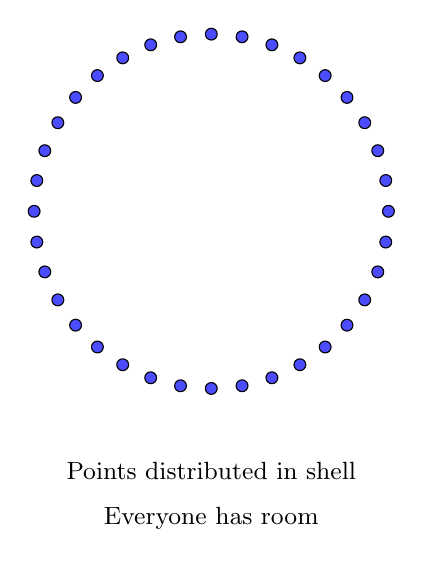
\begin{tikzpicture}[scale=1.5]
% Draw points in a shell pattern
\foreach \i in {0,10,...,350} {
    \draw[fill=blue!70] (\i:1.5cm) circle (0.05cm);
}
% Add label
\node at (0,-2.2) {\small Points distributed in shell};
\node at (0,-2.6) {\small Everyone has room};
\end{tikzpicture}
\end{center}

\column{0.5\textwidth}
\begin{center}
\textbf{Projected to 2D}\\
\vspace{0.3cm}
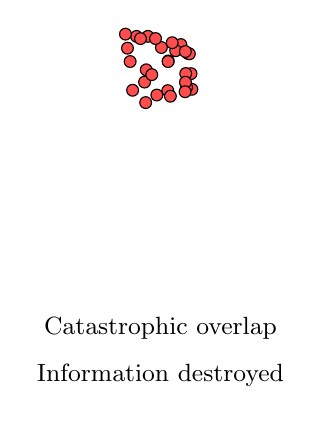
\begin{tikzpicture}[scale=1.5]
% Draw crowded points in center
\foreach \i in {1,...,30} {
    \pgfmathsetmacro\rx{rand*0.3}
    \pgfmathsetmacro\ry{rand*0.3}
    \draw[fill=red!70] (\rx,\ry) circle (0.05cm);
}
% Add label
\node at (0,-2.2) {\small Catastrophic overlap};
\node at (0,-2.6) {\small Information destroyed};
\end{tikzpicture}
\end{center}
\end{columns}

\vspace{0.5cm}
\begin{block}{The Paradox}
Your data lives in 784 dimensions. Your screen has 2.\\
\textbf{How do we preserve the essence when we must destroy the structure?}
\end{block}

\vspace{0.2cm}
\colorbox{yellow!20}{\parbox{0.95\textwidth}{\textbf{Key Insight:} Every visualization is a lie - our job is to make it the most honest lie possible}}
\end{frame}

\begin{frame}{Interactive Demonstration: The Crowding Catastrophe}
\begin{columns}
\column{0.45\textwidth}
\begin{center}
\textbf{High-D Space (10D)}\\
\vspace{0.2cm}
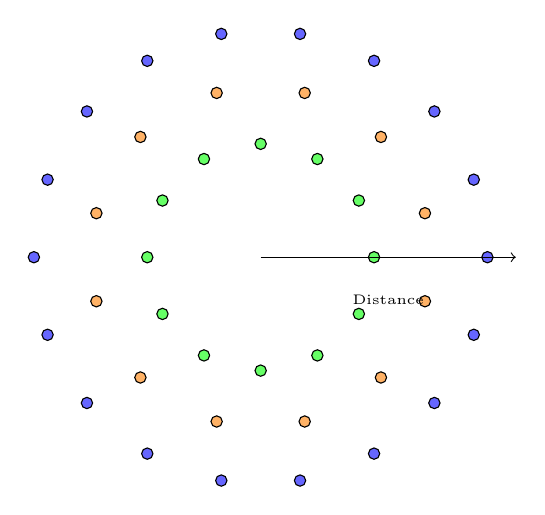
\begin{tikzpicture}[scale=1.8]
% Draw three concentric shells representing different distances
% Inner shell - near neighbors
\foreach \i in {0,30,...,330} {
    \draw[fill=green!60] (\i:0.8cm) circle (0.04cm);
}
% Middle shell - medium distance
\foreach \i in {15,45,...,345} {
    \draw[fill=orange!60] (\i:1.2cm) circle (0.04cm);
}
% Outer shell - far neighbors  
\foreach \i in {0,20,...,340} {
    \draw[fill=blue!60] (\i:1.6cm) circle (0.04cm);
}
\draw[->] (0,0) -- (1.8,0);
\node at (0.9,-0.3) {\tiny Distance};
\end{tikzpicture}
\vspace{0.2cm}

\textbf{Three distinct distance shells}\\
{\small Near \textcolor{green!60}{●} Medium \textcolor{orange!60}{●} Far \textcolor{blue!60}{●}}
\end{center}

\column{0.45\textwidth}
\begin{center}
\textbf{Projected to 2D}\\
\vspace{0.2cm}
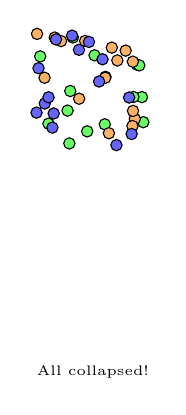
\begin{tikzpicture}[scale=1.8]
% All points compressed to center
\foreach \i in {1,...,15} {
    \pgfmathsetmacro\rx{rand*0.4}
    \pgfmathsetmacro\ry{rand*0.4}
    \draw[fill=green!60] (\rx,\ry) circle (0.04cm);
}
\foreach \i in {1,...,15} {
    \pgfmathsetmacro\rx{rand*0.4}
    \pgfmathsetmacro\ry{rand*0.4}
    \draw[fill=orange!60] (\rx,\ry) circle (0.04cm);
}
\foreach \i in {1,...,15} {
    \pgfmathsetmacro\rx{rand*0.4}
    \pgfmathsetmacro\ry{rand*0.4}
    \draw[fill=blue!60] (\rx,\ry) circle (0.04cm);
}
\node at (0,-2) {\tiny All collapsed!};
\end{tikzpicture}
\vspace{0.2cm}

\textbf{All distances collapse}\\
{\small Cannot distinguish distances}
\end{center}
\end{columns}

\vspace{0.4cm}
\begin{center}
\colorbox{red!20}{\parbox{0.9\textwidth}{\centering\textbf{The Crowding Problem:} Linear projection fails because moderate distances in high-D have no room in 2D}}
\end{center}

\footnotesize\textit{Run interactive\_demo.html to explore this yourself}
\end{frame}

% Slide 4
\begin{frame}{What You Will Master Today: A Complete Journey}
\begin{columns}
\column{0.5\textwidth}
\textbf{Conceptual Mastery}
\begin{itemize}
\item Why information $>$ distance
\item Maximum entropy emergence
\item KL divergence as design choice
\item Crowding as geometric inevitability
\end{itemize}

\textbf{Mathematical Foundation}
\begin{itemize}
\item Derive kernels from principles
\item Gradient as physical forces
\item Prove Student's t necessity
\item Understand convergence
\end{itemize}

\column{0.5\textwidth}
\textbf{Practical Excellence}
\begin{itemize}
\item Debug visually \& quantitatively
\item Choose hyperparameters wisely
\item Validate beyond visualization
\item Recognize failure modes
\end{itemize}

\textbf{Ethical Responsibility}
\begin{itemize}
\item Avoid false pattern creation
\item Communicate limitations
\item Document completely
\item Interpret responsibly
\end{itemize}
\end{columns}

\vspace{0.2cm}
\colorbox{yellow!30}{\textbf{Critical:} Mathematics and visuals will be interwoven, not separated}
\end{frame}

% Slide 5
\begin{frame}{The Paradigm Shift: From Preserving to Accepting Loss}
\begin{center}
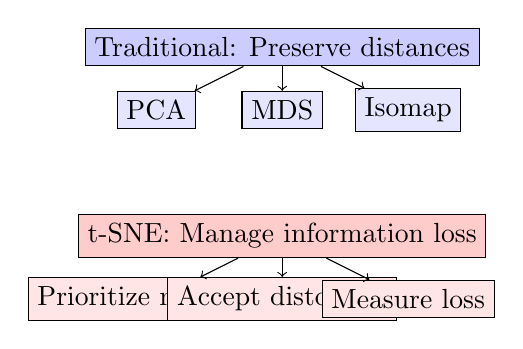
\begin{tikzpicture}[scale=0.8]
% Traditional approach
\node[rectangle, draw, fill=blue!20] (trad) at (0,3) {Traditional: Preserve distances};
\node[rectangle, draw, fill=blue!10] (pca) at (-2,2) {PCA};
\node[rectangle, draw, fill=blue!10] (mds) at (0,2) {MDS};
\node[rectangle, draw, fill=blue!10] (iso) at (2,2) {Isomap};
\draw[->] (trad) -- (pca);
\draw[->] (trad) -- (mds);
\draw[->] (trad) -- (iso);

% t-SNE approach
\node[rectangle, draw, fill=red!20] (tsne) at (0,0) {t-SNE: Manage information loss};
\node[rectangle, draw, fill=red!10] (prior) at (-2,-1) {Prioritize neighbors};
\node[rectangle, draw, fill=red!10] (accept) at (0,-1) {Accept distortion};
\node[rectangle, draw, fill=red!10] (measure) at (2,-1) {Measure loss};
\draw[->] (tsne) -- (prior);
\draw[->] (tsne) -- (accept);
\draw[->] (tsne) -- (measure);
\end{tikzpicture}
\end{center}

\intuition{t-SNE doesn't try to preserve everything - it chooses what to sacrifice}
\end{frame}

% Slide 6
\begin{frame}{Visual Intuition: The Swiss Roll Problem}
\begin{columns}
\column{0.33\textwidth}
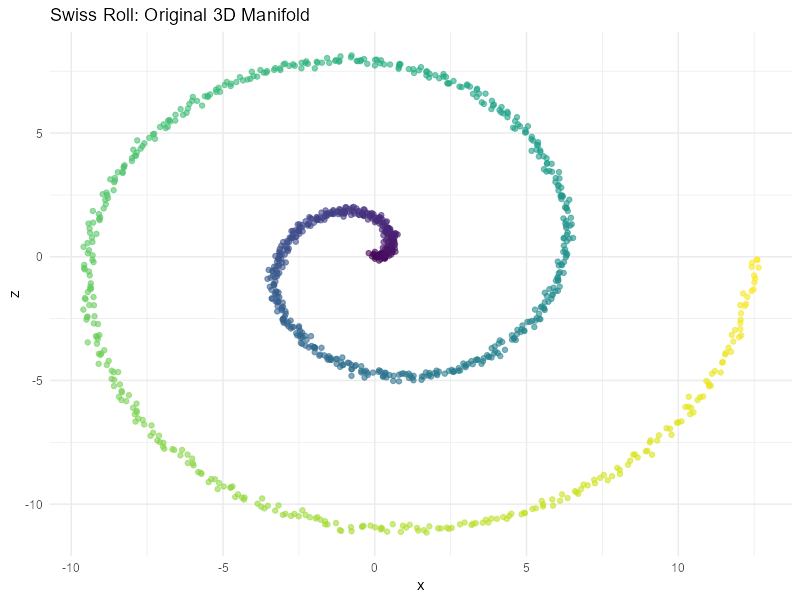
\includegraphics[width=\textwidth]{./Figures/swiss_roll_3d.png}
\textbf{Original Manifold}\\
2D surface in 3D\\
Continuous structure

\column{0.33\textwidth}
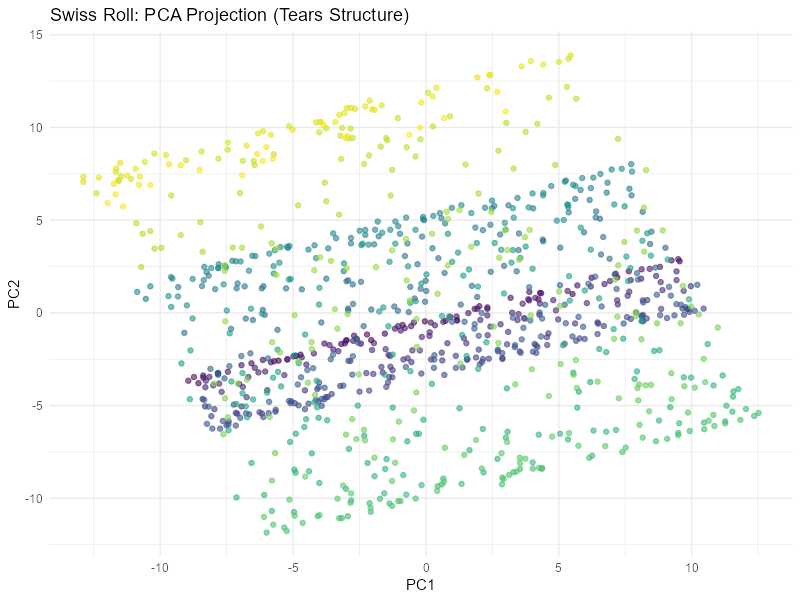
\includegraphics[width=\textwidth]{./Figures/swiss_roll_pca.png}
\textbf{PCA Projection}\\
Tears neighborhoods\\
\textcolor{red}{Destroys continuity}

\column{0.33\textwidth}
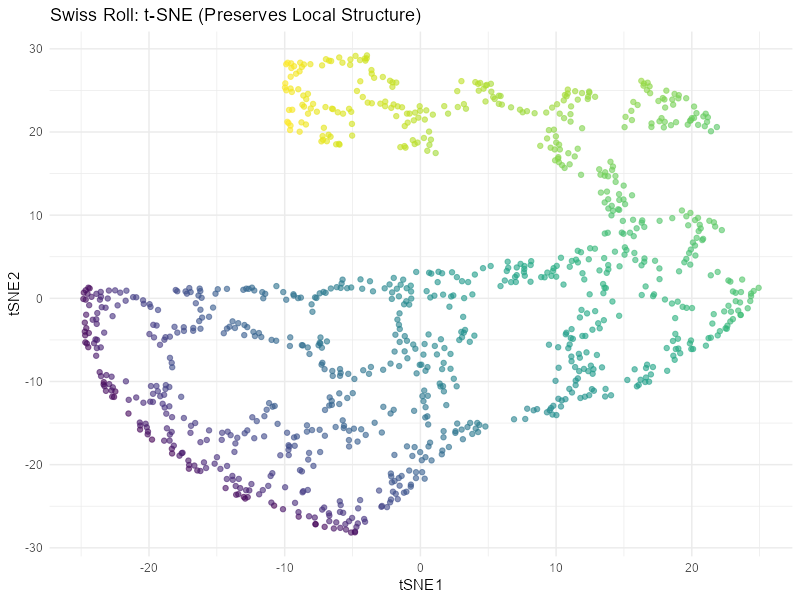
\includegraphics[width=\textwidth]{./Figures/swiss_roll_tsne.png}
\textbf{t-SNE Embedding}\\
Preserves local structure\\
\textcolor{green}{Unfolds naturally}
\end{columns}

\vspace{0.3cm}
\warning{Global structure may be sacrificed for local preservation}
\end{frame}

% Slide 7
\begin{frame}{Why Dimensionality Reduction? Real-World Impact}
\begin{center}
\begin{tikzpicture}
\node at (0,3) {
\includegraphics[width=3cm]{./Figures/genomics_icon.png}};
\node at (4,3) {
\includegraphics[width=3cm]{./Figures/nlp_icon.png}};
\node at (8,3) {
\includegraphics[width=3cm]{./Figures/vision_icon.png}};

\node[text width=3cm, align=center] at (0,1.5) {\textbf{Genomics}\\20,000 genes\\Find disease subtypes};
\node[text width=3cm, align=center] at (4,1.5) {\textbf{NLP}\\50,000 words\\Discover semantics};
\node[text width=3cm, align=center] at (8,1.5) {\textbf{Vision}\\Million pixels\\Reveal patterns};

\draw[->, thick, red] (0,0.5) -- (4,0);
\draw[->, thick, red] (4,0.5) -- (4,0);
\draw[->, thick, red] (8,0.5) -- (4,0);
\node at (4,-0.5) {\textbf{2D Visualization}};
\end{tikzpicture}
\end{center}

\textbf{Common Thread:} Data lives on low-dimensional manifold in high-D space
\end{frame}

% Slide 8
\begin{frame}{The Curse of Dimensionality: A Visual Catastrophe}
\begin{columns}
\column{0.5\textwidth}
\begin{center}
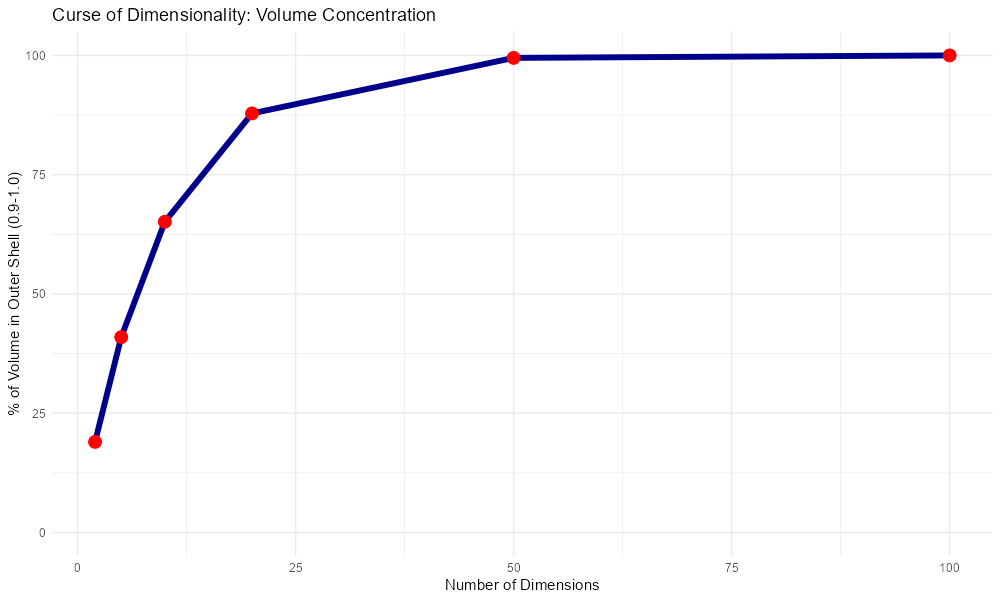
\includegraphics[width=0.9\textwidth]{./Figures/curse_dimensionality_animation.png}
\end{center}
\textbf{Volume in n-D sphere shells:}\\
\small
\begin{tabular}{l|r}
Dimension & Shell (0.9-1.0)\\
\hline
2D & 19\%\\
10D & 65\%\\
100D & 99.997\%\\
1000D & $\approx$100\%
\end{tabular}

\column{0.5\textwidth}
\textbf{Implications:}
\begin{itemize}
\item All points become equidistant
\item Nearest neighbor meaningless
\item Intuition completely fails
\item Traditional metrics break
\end{itemize}

\vspace{0.5cm}
\intuition{In high-D, everything is far from everything else, yet nothing has room}
\end{columns}
\end{frame}

% Slide 9
\begin{frame}{Reframing: From Geometry to Information Theory}
\begin{center}
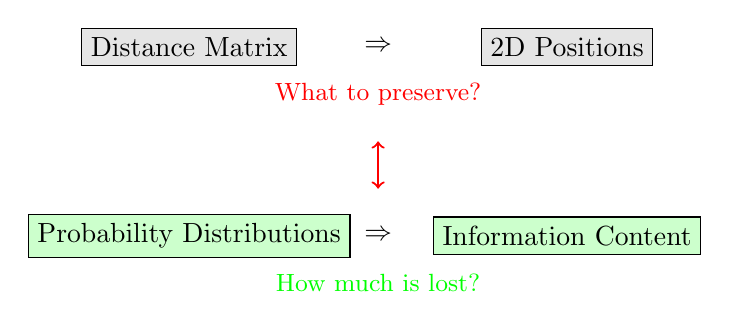
\begin{tikzpicture}[scale=1.2]
% Traditional view
\node[draw, fill=gray!20] (dist) at (0,2) {Distance Matrix};
\node (arrow1) at (2,2) {$\Rightarrow$};
\node[draw, fill=gray!20] (proj) at (4,2) {2D Positions};
\node at (2,1.5) {\textcolor{red}{\small What to preserve?}};

% Information view
\node[draw, fill=green!20] (prob) at (0,0) {Probability Distributions};
\node (arrow2) at (2,0) {$\Rightarrow$};
\node[draw, fill=green!20] (info) at (4,0) {Information Content};
\node at (2,-0.5) {\textcolor{green}{\small How much is lost?}};

\draw[<->, thick, red] (2,1) -- (2,0.5);
\end{tikzpicture}
\end{center}

\begin{block}{The Key Insight}
Instead of asking "How do we preserve distances?"\\
t-SNE asks: "How do we preserve the \textbf{information} about neighborhoods?"
\end{block}
\end{frame}

% Slide 10
\begin{frame}{Information Content: Making It Concrete}
\begin{columns}
\column{0.6\textwidth}
If point $j$ has probability $p_{j|i}$ of being $i$'s neighbor:
\begin{align}
\text{Information: } I(j) &= -\log p_{j|i} \text{ bits}\\
\text{Total entropy: } H(P_i) &= -\sum_j p_{j|i}\log p_{j|i}
\end{align}

\vspace{0.3cm}
\textbf{Example:}
\begin{itemize}
\item Certain neighbor: $p = 1 \Rightarrow I = 0$ bits
\item Likely neighbor: $p = 0.5 \Rightarrow I = 1$ bit
\item Rare neighbor: $p = 0.01 \Rightarrow I = 6.64$ bits
\end{itemize}

\column{0.4\textwidth}

\includegraphics[width=\textwidth]{./Figures/information_visual.png}

\intuition{Surprising events (unlikely neighbors) carry more information}
\end{columns}
\end{frame}

% Slide 11
\begin{frame}{From Distances to Probabilities: Visual Journey}
\begin{center}
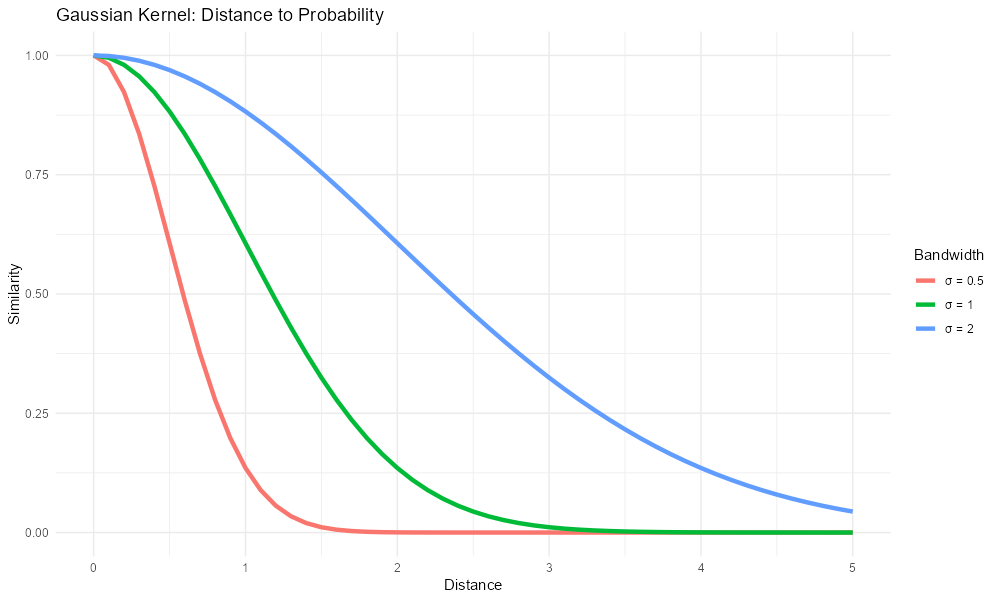
\includegraphics[width=0.9\textwidth]{./Figures/distance_to_probability_animation.png}
\end{center}

\begin{enumerate}
\item Start with distances in high-D space
\item \textbf{Problem:} Same distance means different things in dense vs sparse regions
\item \textbf{Solution:} Adaptive bandwidth Gaussian kernel
\item Convert similarities to probabilities (normalize)
\end{enumerate}

\ethics{This transformation embeds our assumptions about what matters}
\end{frame}

% Slide 12
\begin{frame}{Why Gaussian? Maximum Entropy Derivation}
\begin{block}{The Principle}
Given constraints, choose the \textbf{least biased} distribution
\end{block}

\textbf{Constraints:}
\begin{align}
\sum_j p_{j|i} &= 1 \quad \text{(probability)}\\
\sum_j p_{j|i} d_{ij}^2 &= \sigma_i^2 \quad \text{(expected squared distance)}
\end{align}

\textbf{Optimization:} Maximize $H(P_i) = -\sum_j p_{j|i}\log p_{j|i}$

\textbf{Lagrangian:}
$$\mathcal{L} = H(P_i) + \lambda\left(\sum_j p_{j|i} - 1\right) + \mu\left(\sum_j p_{j|i}d_{ij}^2 - \sigma_i^2\right)$$
\end{frame}

% Slide 13
\begin{frame}{Maximum Entropy Solution: Gaussian Emerges}
Setting $\frac{\partial\mathcal{L}}{\partial p_{j|i}} = 0$:

$$-\log p_{j|i} - 1 + \lambda + \mu d_{ij}^2 = 0$$

Solving for $p_{j|i}$:
$$p_{j|i} = \exp(\lambda - 1) \exp(-\mu d_{ij}^2)$$

After normalization:
$$p_{j|i} = \frac{\exp(-d_{ij}^2/2\sigma_i^2)}{\sum_k \exp(-d_{ik}^2/2\sigma_i^2)}$$

\begin{center}
\colorbox{yellow!30}{\textbf{The Gaussian kernel is not arbitrary - it's mathematically inevitable!}}
\end{center}

\intuition{Maximum entropy $\Rightarrow$ Make no assumptions beyond what you know}
\end{frame}

% Slide 14
\begin{frame}{Adaptive Bandwidth: The Local Density Solution}
\begin{columns}
\column{0.5\textwidth}
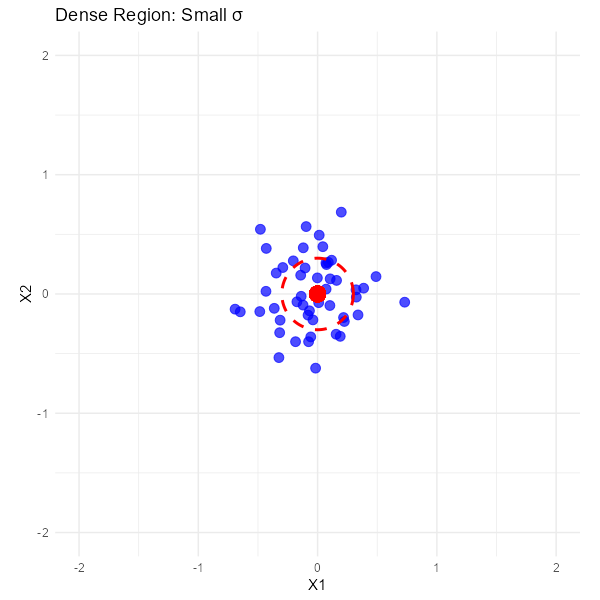
\includegraphics[width=\textwidth]{./Figures/adaptive_bandwidth_dense.png}
\textbf{Dense Region}\\
Small $\sigma_i$ captures many neighbors

\column{0.5\textwidth}
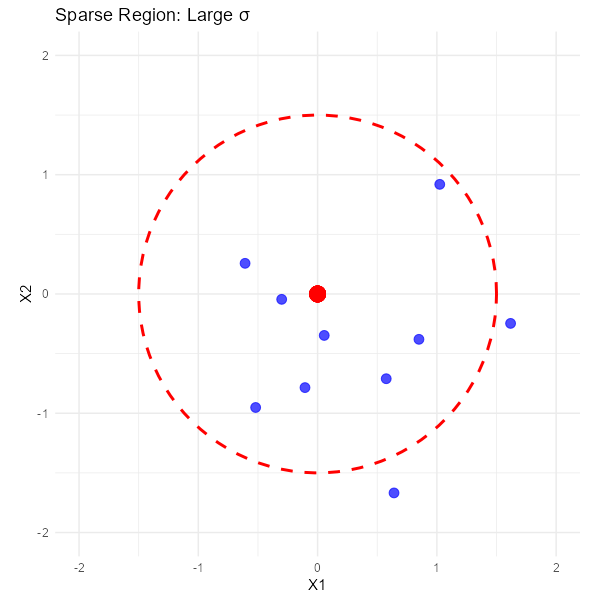
\includegraphics[width=\textwidth]{./Figures/adaptive_bandwidth_sparse.png}
\textbf{Sparse Region}\\
Large $\sigma_i$ reaches distant points
\end{columns}

\vspace{0.3cm}
\textbf{The Problem:} How to set thousands of $\sigma_i$ values?\\
\textbf{The Solution:} Perplexity - one intuitive parameter for all!

\warning{Fixed bandwidth would oversimplify dense regions or fragment sparse ones}
\end{frame}

% Slide 15
\begin{frame}{Perplexity: The Intuitive Control Parameter}
\begin{block}{Definition}
$$\text{Perp}(P_i) = 2^{H(P_i)}$$
where $H(P_i) = -\sum_j p_{j|i}\log_2 p_{j|i}$ is entropy in bits
\end{block}

\begin{columns}
\column{0.5\textwidth}
\textbf{Interpretation:}
\begin{itemize}
\item Perp = 30 $\approx$ "30 effective neighbors"
\item Automatically adapts $\sigma_i$ per point
\item Binary search finds right $\sigma_i$
\end{itemize}

\column{0.5\textwidth}
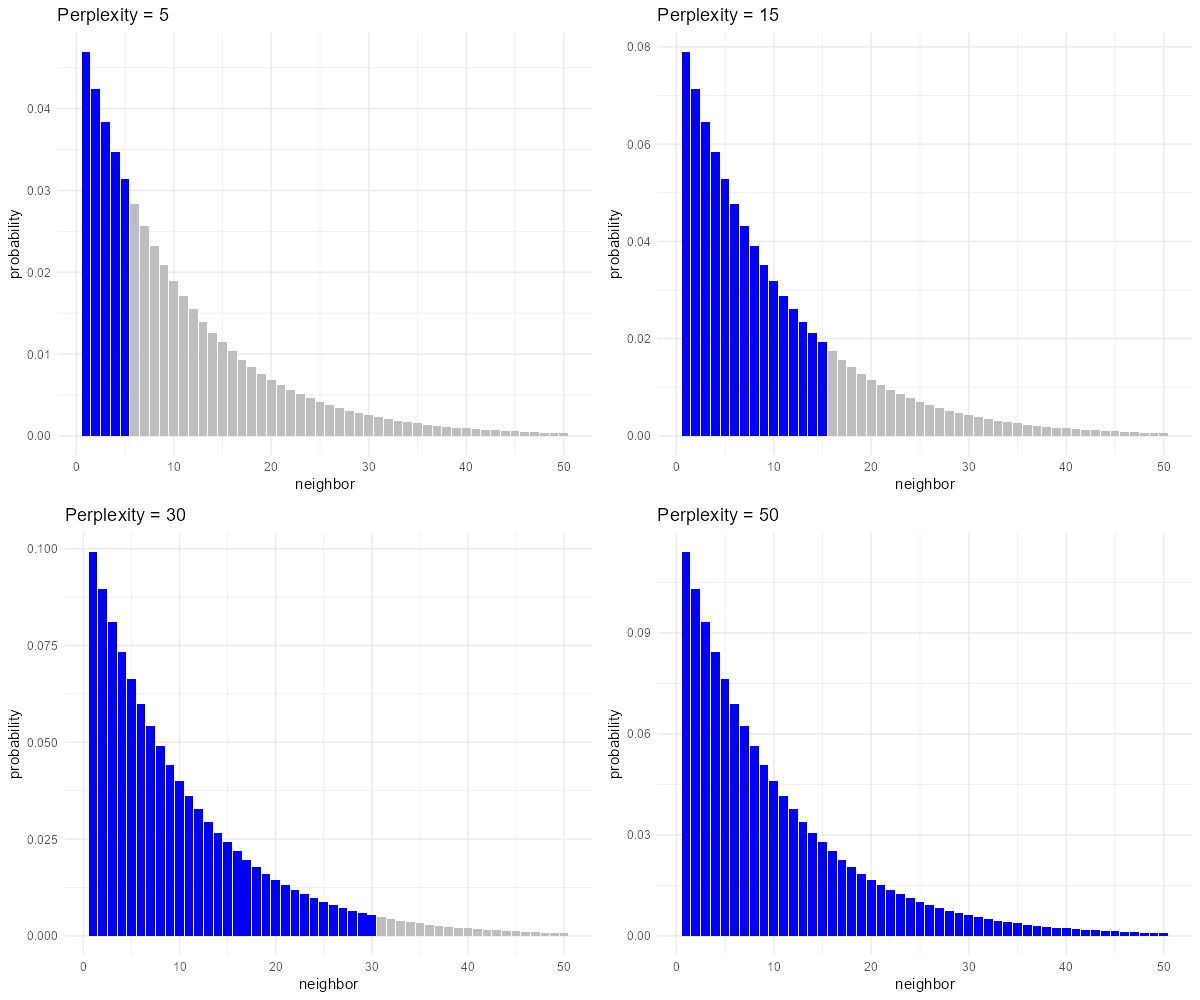
\includegraphics[width=\textwidth]{./Figures/perplexity_visual.png}
\end{columns}

\intuition{Perplexity is "how many neighbors should each point care about"}
\end{frame}

% Slide 16
\begin{frame}{Algorithm: Finding $\sigma_i$ via Binary Search}
\begin{algorithm}[H]
\caption{Adaptive Bandwidth Selection}
\begin{algorithmic}[1]
\FOR{each point $i$}
\STATE target\_perp $\leftarrow$ user\_specified
\STATE $\sigma_{min} \leftarrow 0$, $\sigma_{max} \leftarrow \infty$
\WHILE{not converged}
\STATE $\sigma_i \leftarrow (\sigma_{min} + \sigma_{max})/2$
\STATE Compute $p_{j|i}$ using current $\sigma_i$
\STATE current\_perp $\leftarrow 2^{H(P_i)}$
\IF{current\_perp $>$ target\_perp}
\STATE $\sigma_{max} \leftarrow \sigma_i$ \COMMENT{Too many neighbors}
\ELSE
\STATE $\sigma_{min} \leftarrow \sigma_i$ \COMMENT{Too few neighbors}
\ENDIF
\ENDWHILE
\ENDFOR
\end{algorithmic}
\end{algorithm}
\end{frame}

% Slide 17
\begin{frame}{Measuring Information Loss: KL Divergence}
\begin{columns}
\column{0.6\textwidth}
\textbf{Cross-Entropy:} Bits using wrong distribution
$$H(P,Q) = -\sum_j p_j \log q_j$$

\textbf{KL Divergence:} Extra bits from using $Q$ instead of $P$
$$\text{KL}(P||Q) = \sum_j p_j \log\frac{p_j}{q_j}$$

\textbf{Critical Asymmetry:}
\begin{itemize}
\item Miss a neighbor: $p=0.3, q=0.01$\\
Penalty: $0.3 \log(30) \approx 1.02$ bits
\item False neighbor: $p=0.01, q=0.3$\\
Penalty: $0.01 \log(0.033) \approx -0.035$ bits
\end{itemize}

\column{0.4\textwidth}
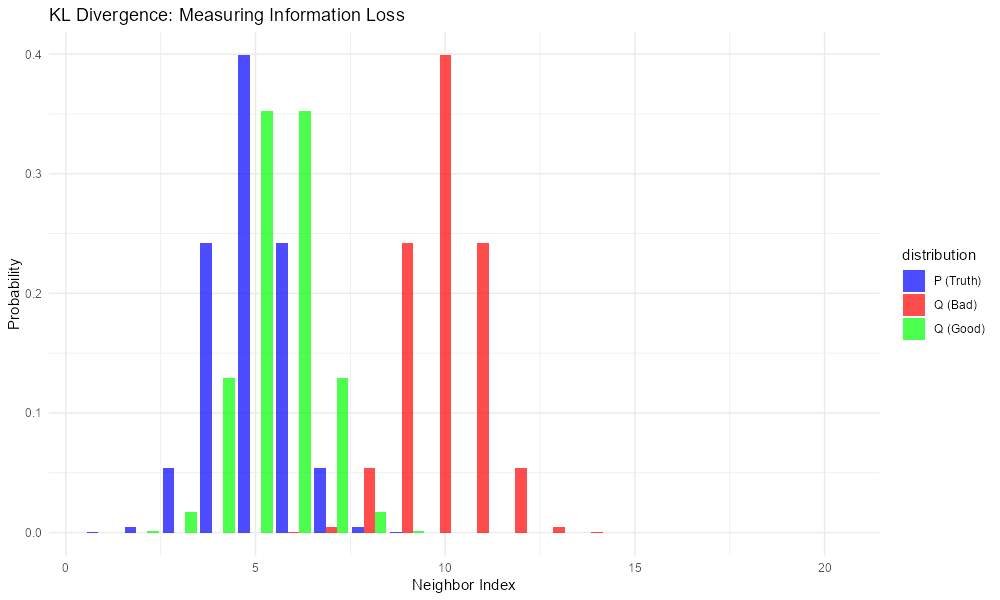
\includegraphics[width=\textwidth]{./Figures/kl_divergence_asymmetry.png}

\colorbox{red!20}{t-SNE heavily penalizes\\separating true neighbors!}
\end{columns}
\end{frame}

% Slide 18
\begin{frame}{Visual KL Divergence: What We're Minimizing}
\begin{center}
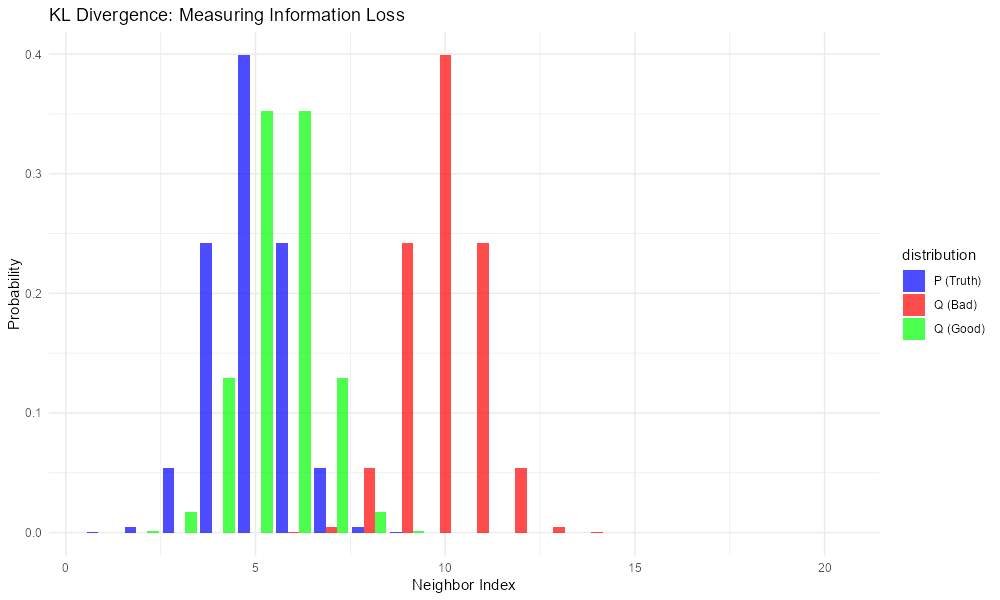
\includegraphics[width=0.9\textwidth]{./Figures/kl_divergence_visualization.png}
\end{center}

\begin{itemize}
\item \textbf{Blue bars:} High-D probability distribution $P_i$
\item \textbf{Red bars:} Low-D probability distribution $Q_i$
\item \textbf{Yellow area:} KL divergence (information lost)
\end{itemize}

\intuition{We're trying to make the red bars match the blue bars, but we care more about missing blues than extra reds}
\end{frame}

% Slide 19
\begin{frame}{The Original SNE Algorithm}
\begin{columns}
\column{0.5\textwidth}
\textbf{High-D Similarities:}
$$p_{j|i} = \frac{\exp(-\|x_i-x_j\|^2/2\sigma_i^2)}{\sum_k \exp(-\|x_i-x_k\|^2/2\sigma_i^2)}$$

\textbf{Low-D Similarities:}
$$q_{j|i} = \frac{\exp(-\|y_i-y_j\|^2)}{\sum_k \exp(-\|y_i-y_k\|^2)}$$
Note: Fixed variance = 1 in low-D

\column{0.5\textwidth}
\textbf{Cost Function:}
$$C = \sum_i \text{KL}(P_i||Q_i)$$

\textbf{Gradient Descent:}
$$\frac{\partial C}{\partial y_i} = 2\sum_j (p_{j|i} - q_{j|i})(y_i - y_j)$$

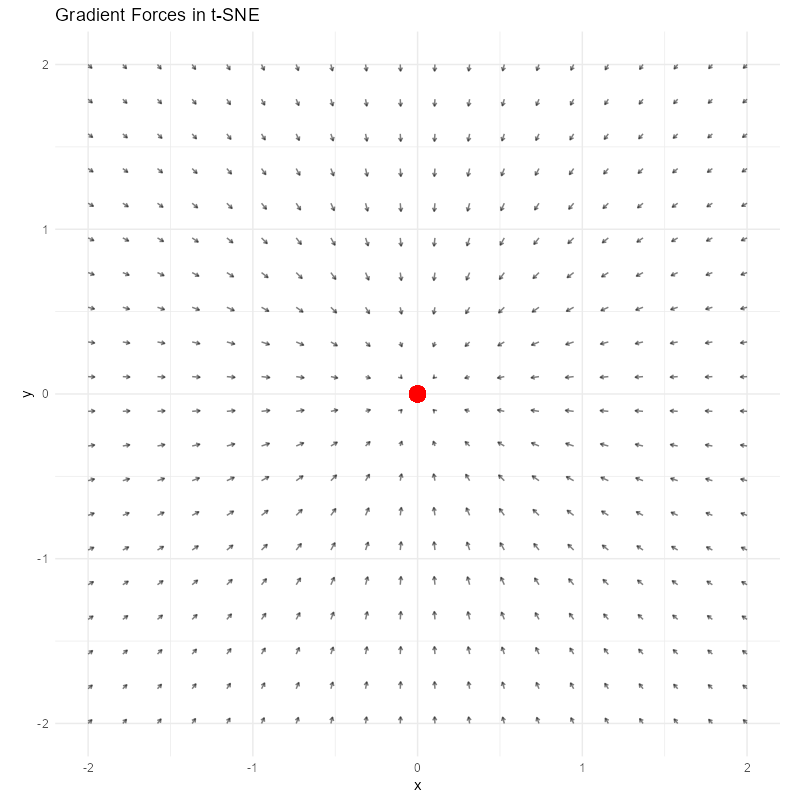
\includegraphics[width=\textwidth]{./Figures/sne_gradient_forces.png}
\end{columns}
\end{frame}

% Slide 20
\begin{frame}{SNE's Fatal Flaw: The Crowding Problem Visualized}
\begin{center}
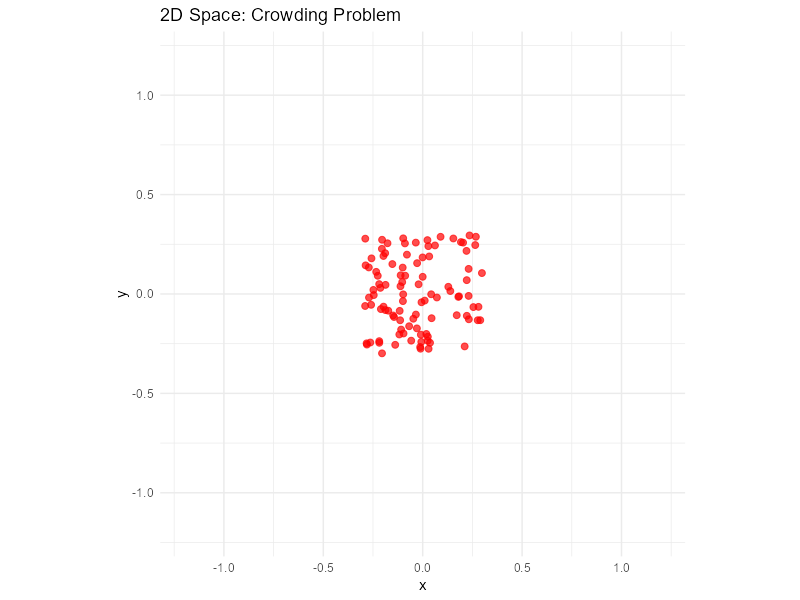
\includegraphics[width=0.8\textwidth]{./Figures/crowding_problem_animation.png}
\end{center}

\begin{columns}
\column{0.5\textwidth}
\textbf{In 10D:} Points at moderate distances\\
(0.5 - 0.8 from center)\\
Plenty of room in shell

\column{0.5\textwidth}
\textbf{In 2D:} Same distances impossible\\
Area grows as $r^2$ not $r^{10}$\\
\textcolor{red}{Moderate distances crushed!}
\end{columns}

\warning{Gaussian tails decay too fast to represent moderate distances}
\end{frame}

% Slide 21
\begin{frame}{The Brilliant Solution: Student's t-Distribution}
\begin{columns}
\column{0.5\textwidth}
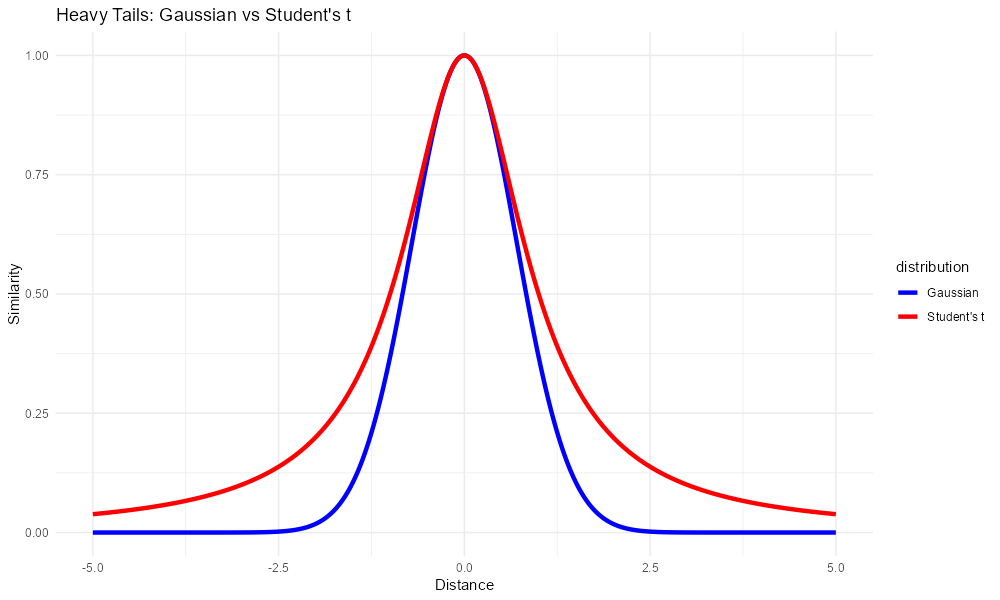
\includegraphics[width=\textwidth]{./Figures/gaussian_vs_t_comparison.png}

\textbf{Mathematical Forms:}\\
Gaussian: $\propto e^{-d^2}$\\
Student's t: $\propto (1+d^2)^{-1}$

\column{0.5\textwidth}
\textbf{Key Differences:}
\begin{itemize}
\item Polynomial vs exponential decay
\item Heavy tails = more "room"
\item Moderate distances preserved
\item Natural repulsion at distance
\end{itemize}

\intuition{Think of it as creating "virtual space" that doesn't exist in 2D}
\end{columns}

\vspace{0.3cm}
\colorbox{green!20}{\textbf{Van der Maaten \& Hinton (2008):} Use different kernels for different spaces!}
\end{frame}

% Slide 22
\begin{frame}{Why Student's t? Quantitative Analysis}
\begin{columns}
\column{0.6\textwidth}
\textbf{Similarity Ratio at Different Distances:}

For $d_1 = 1$ and $d_2 = 3$:

\textbf{Gaussian:}
$$\frac{q(d_1)}{q(d_2)} = \frac{e^{-1}}{e^{-9}} = e^8 \approx 2981$$

\textbf{Student's t:}
$$\frac{q(d_1)}{q(d_2)} = \frac{1/(1+1)}{1/(1+9)} = 5$$

\column{0.4\textwidth}
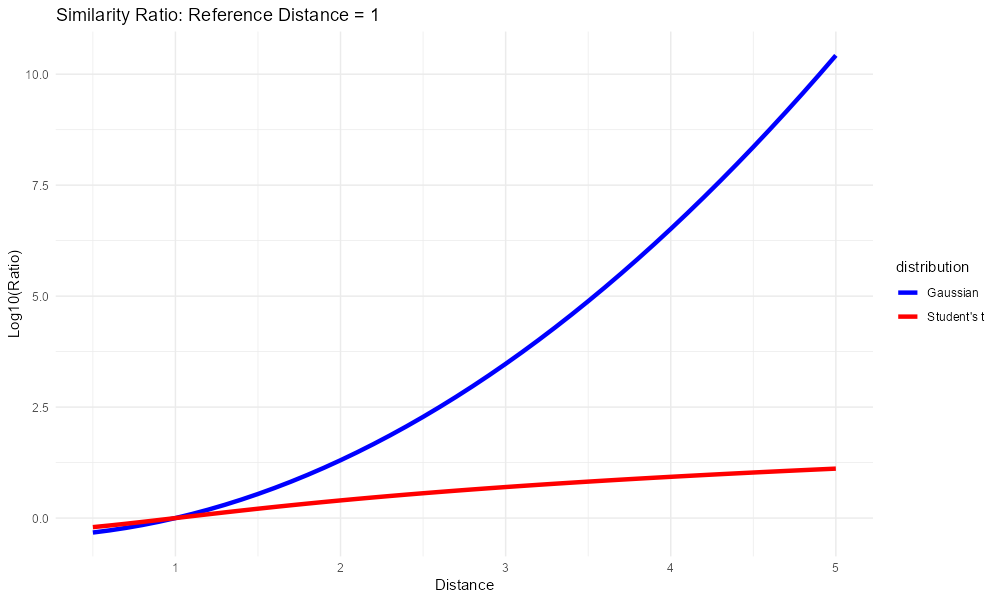
\includegraphics[width=\textwidth]{./Figures/distance_ratio_plot.png}

\colorbox{yellow!30}{600× difference in\\representation capacity!}
\end{columns}

\warning{This is why SNE fails - it literally runs out of space}
\end{frame}

% Slide 23
\begin{frame}{Visual Proof: How Heavy Tails Solve Crowding}
\begin{center}

\includegraphics[width=0.9\textwidth]{./Figures/heavy_tails_solution_animation.png}
\end{center}

\begin{itemize}
\item \textbf{Left:} SNE with Gaussian - points crushed together
\item \textbf{Right:} t-SNE with Student's t - natural separation
\item \textbf{Key:} Heavy tails allow moderate distances without penalty
\end{itemize}

\intuition{Heavy tails act like a "pressure valve" for crowded points}
\end{frame}

% Slide 24
\begin{frame}{The t-SNE Algorithm: Complete Specification}
\begin{block}{Key Modifications from SNE}
\begin{enumerate}
\item \textbf{Symmetrized:} $p_{ij} = \frac{p_{j|i} + p_{i|j}}{2n}$ (simplifies gradient)
\item \textbf{Student's t in low-D:} $q_{ij} \propto (1 + \|y_i - y_j\|^2)^{-1}$
\item \textbf{Single KL:} $C = \text{KL}(P||Q)$ not $\sum_i \text{KL}(P_i||Q_i)$
\end{enumerate}
\end{block}

\textbf{Complete Cost Function:}
$$C = \sum_{i,j} p_{ij} \log\frac{p_{ij}}{q_{ij}}$$

where $q_{ij} = \frac{(1 + \|y_i - y_j\|^2)^{-1}}{\sum_{k,l} (1 + \|y_k - y_l\|^2)^{-1}}$
\end{frame}

% Slide 25
\begin{frame}{The t-SNE Gradient: Mathematical Elegance}
\textbf{The Gradient:}
$$\frac{\partial C}{\partial y_i} = 4\sum_j (p_{ij} - q_{ij})(y_i - y_j)(1 + \|y_i - y_j\|^2)^{-1}$$

\begin{center}
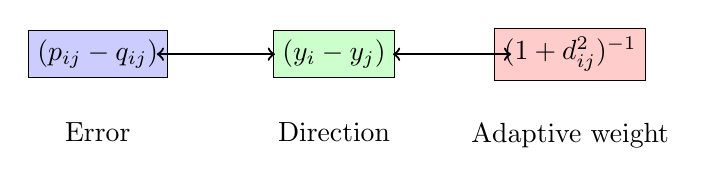
\begin{tikzpicture}[scale=1.5]
\node[draw, fill=blue!20] (pq) at (0,0) {$(p_{ij} - q_{ij})$};
\node[draw, fill=green!20] (dir) at (2,0) {$(y_i - y_j)$};
\node[draw, fill=red!20] (weight) at (4,0) {$(1 + d_{ij}^2)^{-1}$};

\node[below] at (0,-0.5) {Error};
\node[below] at (2,-0.5) {Direction};
\node[below] at (4,-0.5) {Adaptive weight};

\draw[<->, thick] (0.5,0) -- (1.5,0);
\draw[<->, thick] (2.5,0) -- (3.5,0);
\end{tikzpicture}
\end{center}

\intuition{Forces get weaker with distance, preventing distant clusters from merging}
\end{frame}

% Slide 26
\begin{frame}{Visualizing the Gradient as Forces}
\begin{center}
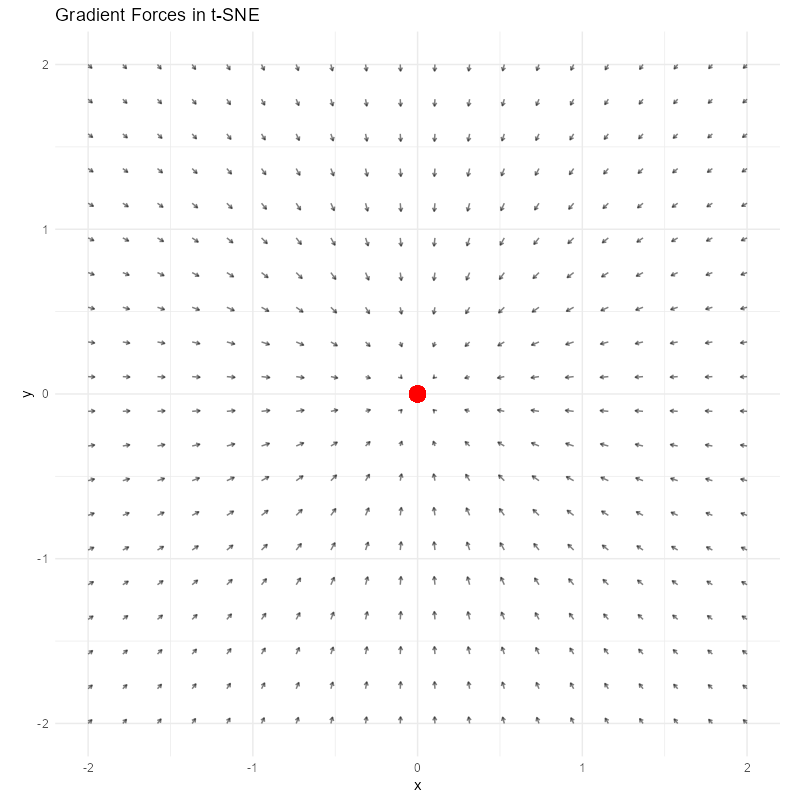
\includegraphics[width=0.8\textwidth]{./Figures/gradient_force_field.png}
\end{center}

\begin{columns}
\column{0.5\textwidth}
\textbf{Attractive Forces:}\\
When $p_{ij} > q_{ij}$\\
Pull points together\\
Preserve neighborhoods

\column{0.5\textwidth}
\textbf{Repulsive Forces:}\\
When $p_{ij} < q_{ij}$\\
Push points apart\\
Create space
\end{columns}

\ethics{The algorithm literally simulates physical forces - misunderstanding this leads to misinterpretation}
\end{frame}

% Slide 27
\begin{frame}{Pseudo-code: The Core Optimization Loop}
\begin{algorithm}[H]
\caption{t-SNE Core Loop}
\begin{algorithmic}[1]
\STATE \textbf{Input:} $X \in \mathbb{R}^{n \times D}$, perplexity, T = 1000
\STATE Compute $P$ matrix using adaptive Gaussian
\STATE Symmetrize: $p_{ij} = (p_{j|i} + p_{i|j})/2n$
\STATE Initialize $Y \sim \mathcal{N}(0, 10^{-4}I)$
\FOR{$t = 1$ to $T$}
\STATE Compute $Q$ matrix using Student's t
\IF{$t < 250$} 
\STATE $P_{exag} = 4 \cdot P$ \COMMENT{Early exaggeration}
\ENDIF
\STATE $\nabla C = 4\sum_j (p_{ij} - q_{ij})(y_i - y_j)/(1 + d_{ij}^2)$
\STATE $Y^{(t)} = Y^{(t-1)} - \eta\nabla C + \alpha(Y^{(t-1)} - Y^{(t-2)})$
\STATE Adapt learning rate based on gradient sign changes
\ENDFOR
\RETURN $Y$
\end{algorithmic}
\end{algorithm}
\end{frame}

% Slide 28
\begin{frame}{Optimization Tricks: Making t-SNE Work}
\begin{columns}
\column{0.5\textwidth}
\textbf{1. Early Exaggeration}
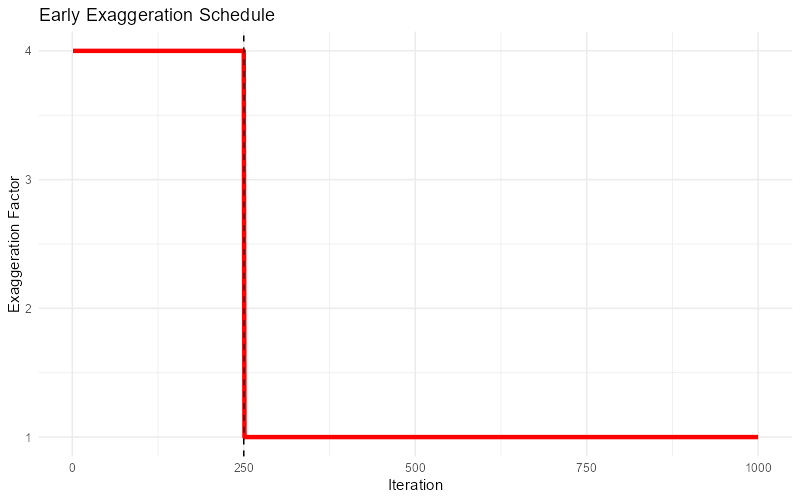
\includegraphics[width=\textwidth]{./Figures/early_exaggeration.png}
Multiply $P$ by 4 for first 250 iterations\\
Forms tight clusters early

\column{0.5\textwidth}
\textbf{2. Momentum Schedule}
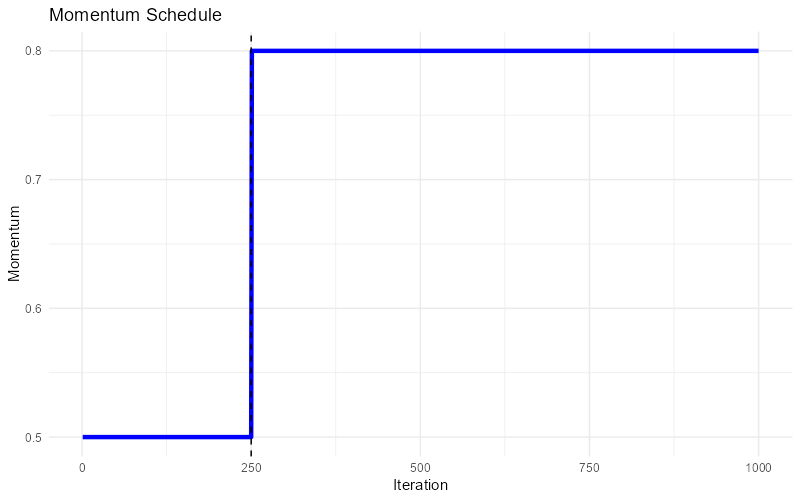
\includegraphics[width=\textwidth]{./Figures/momentum_schedule.png}
$\alpha = 0.5 \to 0.8$ at iteration 250\\
Escapes local minima
\end{columns}

\vspace{0.3cm}
\textbf{3. Adaptive Learning Rate:}
If gradient keeps same sign: $\eta \times 1.2$\\
If gradient changes sign: $\eta \times 0.8$

\intuition{These tricks reduce runtime from hours to minutes!}
\end{frame}

% Slide 29
\begin{frame}{Numerical Stability: Critical Implementation Details}
\begin{block}{Common Numerical Issues and Solutions}
\begin{enumerate}
\item \textbf{Log of zero:} Add $\epsilon = 10^{-12}$ to all probabilities
\item \textbf{Exponential overflow:} Use log-sum-exp trick:
$$\log\sum_i e^{x_i} = \max(x) + \log\sum_i e^{x_i - \max(x)}$$
\item \textbf{Division by zero:} Add $\epsilon$ to all squared distances
\item \textbf{Gradient explosion:} Clip if $\|\nabla\| > 100$
\item \textbf{Duplicate points:} Add small noise or remove
\end{enumerate}
\end{block}

\warning{Ignoring these causes NaN values and crashes!}

\textbf{Memory Optimization:} Use sparse $P$ matrix (only k-NN stored)
\end{frame}

% Slide 30
\begin{frame}{Barnes-Hut Approximation: From $O(n^2)$ to $O(n\log n)$}
\begin{columns}
\column{0.5\textwidth}
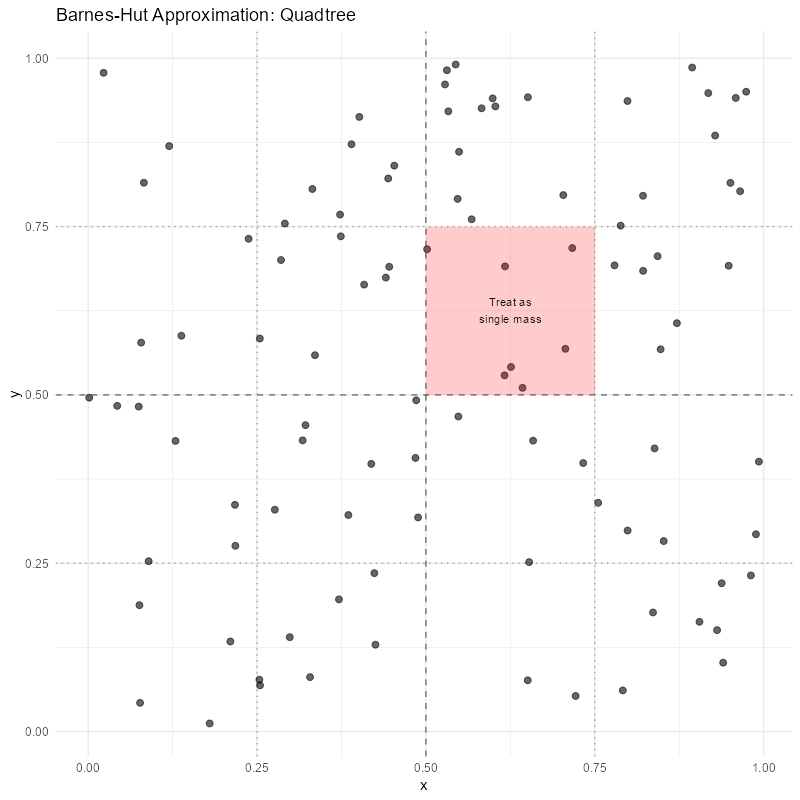
\includegraphics[width=\textwidth]{./Figures/barnes_hut_tree.png}

\textbf{Key Idea:}\\
Treat distant point clusters as single mass

\column{0.5\textwidth}
\textbf{Criterion:}
$$\frac{r_{cell}}{d_{to\_cell}} < \theta$$

\begin{itemize}
\item $\theta = 0$: Exact (slow)
\item $\theta = 0.5$: Good balance
\item $\theta = 1$: Fast (inaccurate)
\end{itemize}

\textbf{Speedup:}\\
10K points: 50× faster\\
100K points: 200× faster
\end{columns}

\intuition{Most computation is repulsive forces between distant points - approximate them!}
\end{frame}

% Slide 31
\begin{frame}{Debugging t-SNE: Visual Diagnosis Guide}
\begin{center}
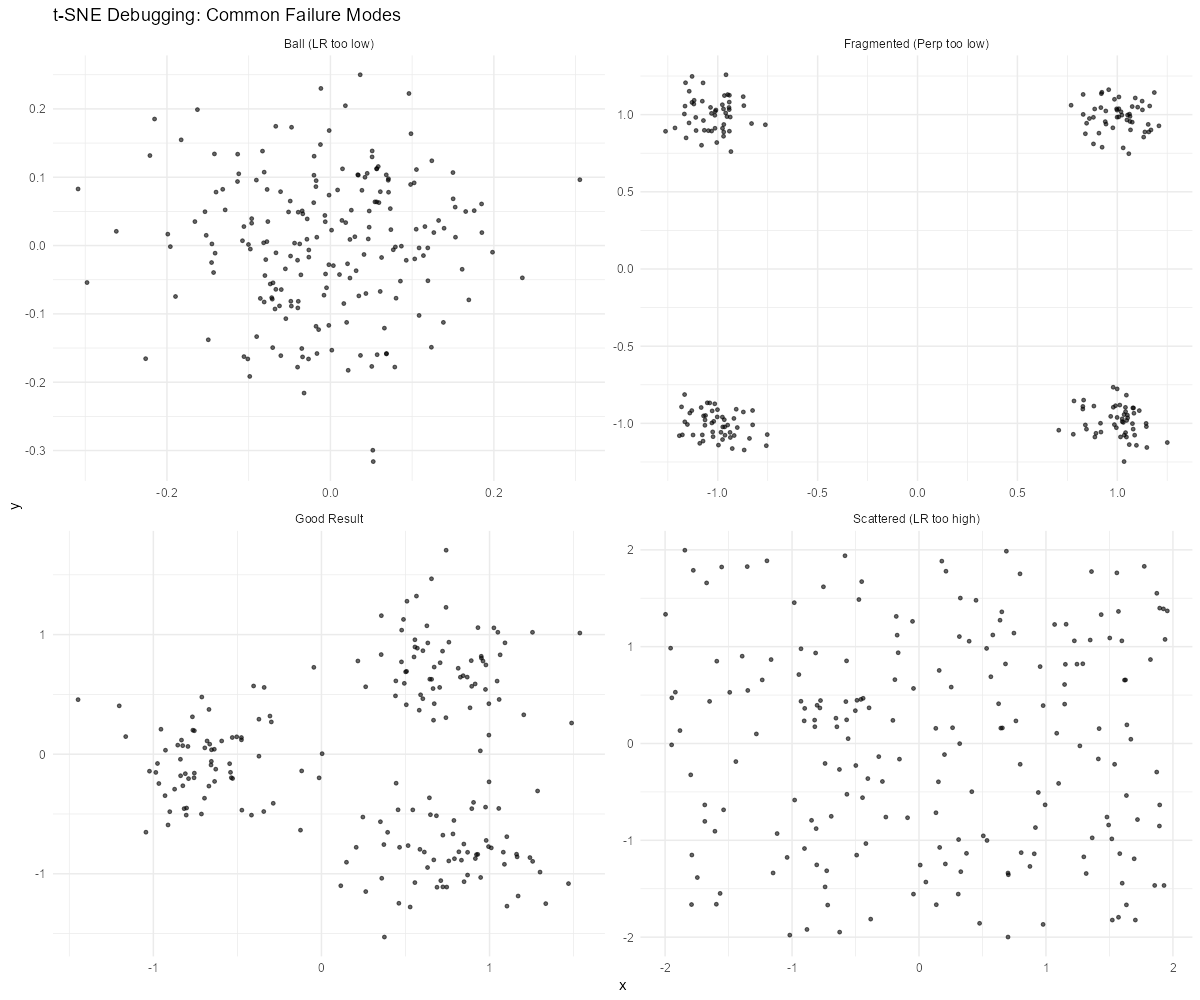
\includegraphics[width=0.9\textwidth]{./Figures/debugging_visual_guide.png}
\end{center}

\begin{tabular}{l|l|l}
\textbf{Symptom} & \textbf{Cause} & \textbf{Fix}\\
\hline
Ball of points & Learning rate too low & Increase $\eta$\\
Scattered points & Learning rate too high & Decrease $\eta$\\
Fragmented clusters & Perplexity too low & Increase perplexity\\
No structure & Too few iterations & Increase T\\
Different each run & Not converged & More iterations
\end{tabular}

\ethics{Always run multiple times - single runs can be misleading!}
\end{frame}

% Slide 32
\begin{frame}{Perplexity Deep Dive: Your Main Control}
\begin{center}
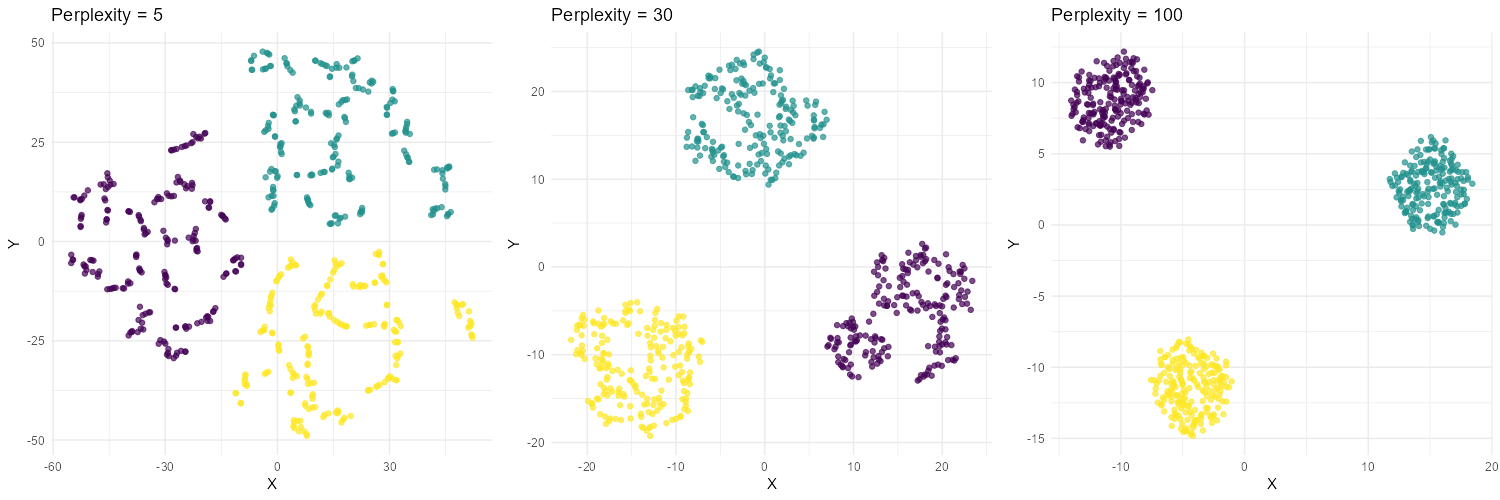
\includegraphics[width=0.9\textwidth]{./Figures/perplexity_comparison.png}
\end{center}

\begin{columns}
\column{0.33\textwidth}
\textbf{Perp = 5}\\
Very local focus\\
Many fragments\\
Good for outliers

\column{0.33\textwidth}
\textbf{Perp = 30}\\
Balanced view\\
Clear clusters\\
Most common choice

\column{0.33\textwidth}
\textbf{Perp = 100}\\
Global structure\\
Merges clusters\\
Loses detail
\end{columns}

\warning{Truth is what's consistent across multiple perplexity values}
\end{frame}

% Slide 33
\begin{frame}{Critical: What You CANNOT Interpret}
\begin{center}
\colorbox{red!30}{\Large\textbf{The Three Deadly Sins of t-SNE Interpretation}}
\end{center}

\begin{columns}
\column{0.33\textwidth}
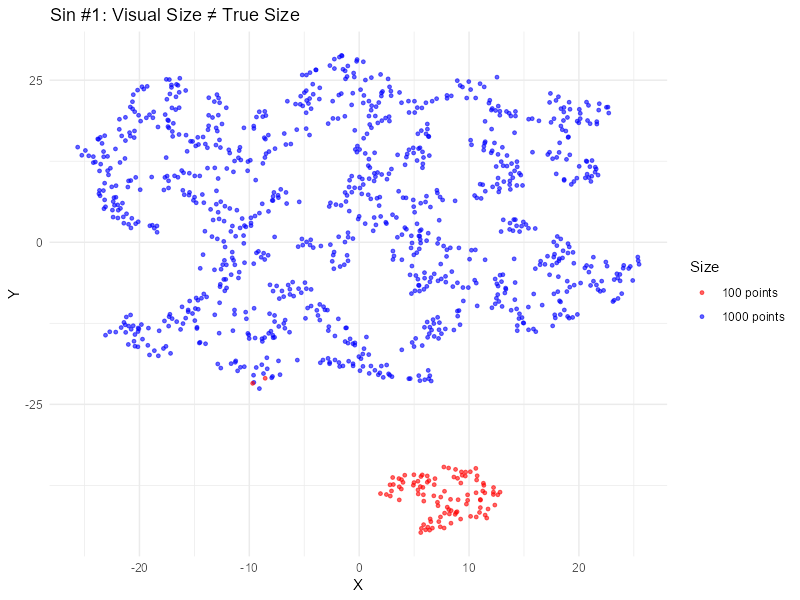
\includegraphics[width=\textwidth]{./Figures/sin1_cluster_size.png}
\textbf{Sin \#1: Cluster Sizes}\\
1000 vs 100 points\\
Look same size!

\column{0.33\textwidth}
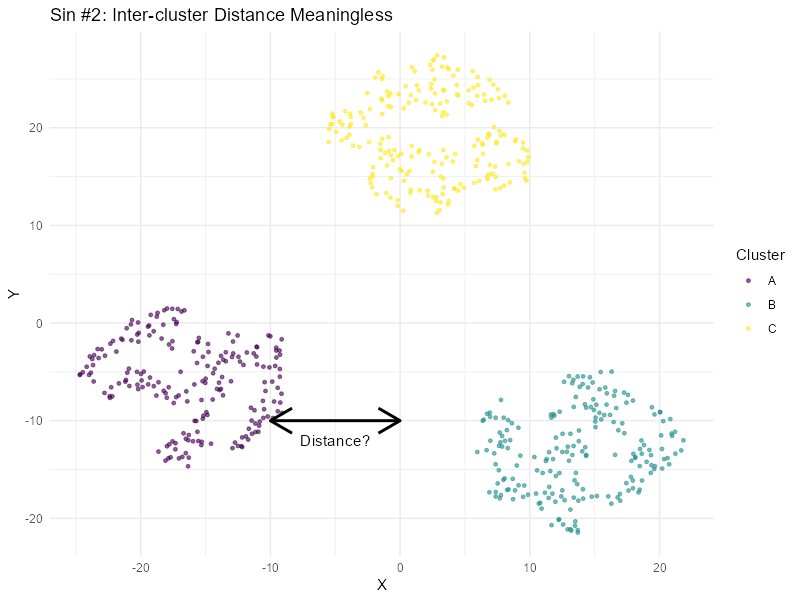
\includegraphics[width=\textwidth]{./Figures/sin2_distances.png}
\textbf{Sin \#2: Inter-cluster Distance}\\
Gap size meaningless\\
No global coordinates

\column{0.33\textwidth}
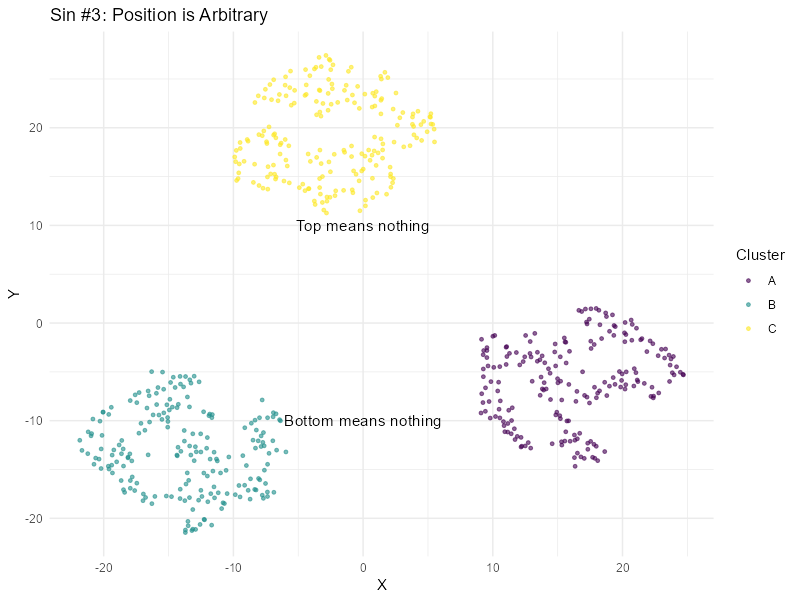
\includegraphics[width=\textwidth]{./Figures/sin3_position.png}
\textbf{Sin \#3: Absolute Position}\\
Top vs bottom\\
Rotation arbitrary
\end{columns}

\vspace{0.3cm}
\colorbox{green!30}{\textbf{What you CAN trust:} Local neighborhoods and cluster separation}
\end{frame}

% Slide 34
\begin{frame}{Case Study: MNIST Digits - Complete Pipeline}
\begin{columns}
\column{0.5\textwidth}
\textbf{Data:}
\begin{itemize}
\item 70,000 handwritten digits
\item 28×28 = 784 dimensions
\item 10 classes (0-9)
\end{itemize}

\textbf{Pipeline:}
\begin{enumerate}
\item Scale pixels to [0,1]
\item PCA to 50D (95\% variance)
\item Remove outliers (>3σ)
\item t-SNE with perp=30
\item Validate with NPr metric
\end{enumerate}

\column{0.5\textwidth}
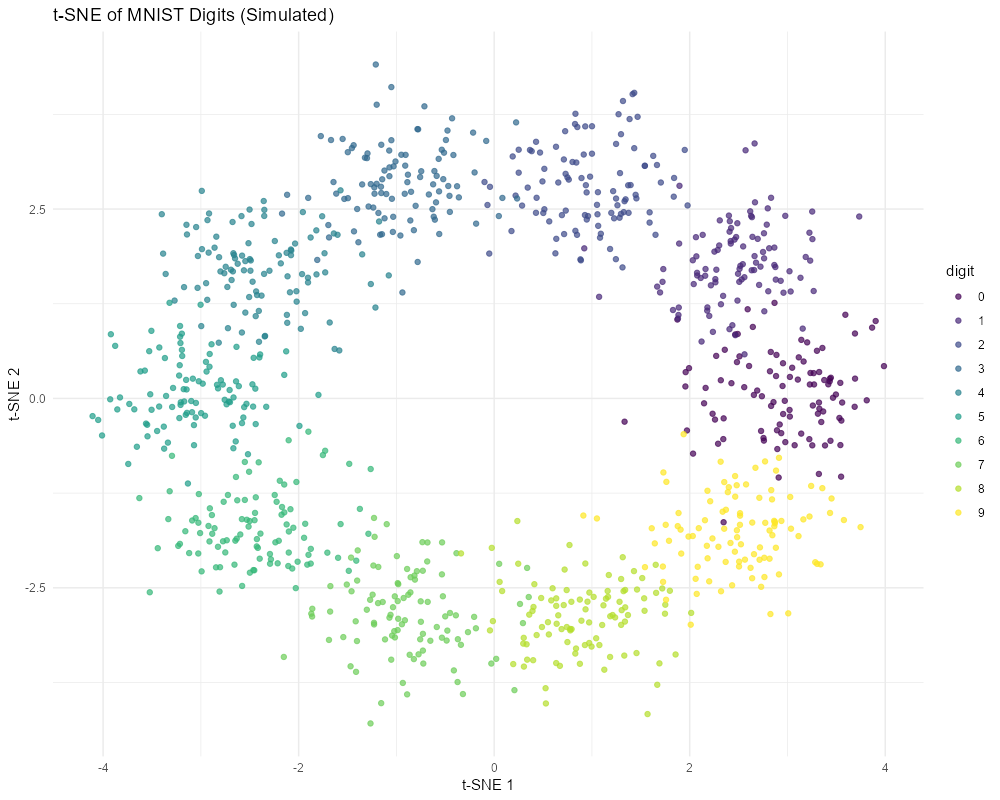
\includegraphics[width=\textwidth]{./Figures/mnist_tsne_result.png}

\textbf{Observations:}
\begin{itemize}
\item Clear digit separation
\item 4-9 proximity (visual similarity)
\item Sub-clusters = writing styles
\end{itemize}
\end{columns}

\textit{Run tsne\_mnist.R for full analysis}
\end{frame}

% Slide 35
\begin{frame}{Validation: Beyond Visual Inspection}
\begin{block}{Quantitative Validation Metrics}
\textbf{1. Neighborhood Preservation (NPr):}
$$\text{NPr}(k) = \frac{1}{n}\sum_i \frac{|N_k^{high}(i) \cap N_k^{low}(i)|}{k}$$

\textbf{2. Trustworthiness:}
$$T(k) = 1 - \frac{2}{nk(2n-3k-1)}\sum_i \sum_{j \in U_k(i)} (r(i,j) - k)$$

\textbf{3. Continuity:}
$$C(k) = 1 - \frac{2}{nk(2n-3k-1)}\sum_i \sum_{j \in V_k(i)} (r'(i,j) - k)$$
\end{block}

\warning{Never publish t-SNE without these metrics!}
\end{frame}

% Slide 36
\begin{frame}{Stability Analysis: How Reliable Is Your Embedding?}
\begin{columns}
\column{0.5\textwidth}
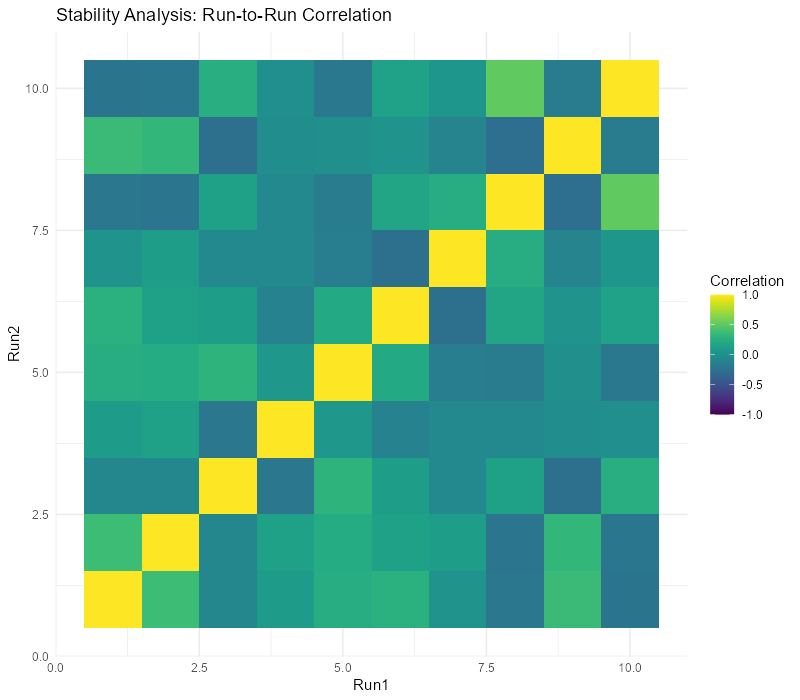
\includegraphics[width=\textwidth]{./Figures/stability_analysis.png}

\textbf{Protocol:}
\begin{enumerate}
\item Run t-SNE 10 times
\item Different random seeds
\item Compute pairwise correlations
\item Report mean ± std
\end{enumerate}

\column{0.5\textwidth}
\textbf{Interpretation:}
\begin{itemize}
\item $r > 0.9$: Very stable
\item $r = 0.7-0.9$: Moderately stable
\item $r < 0.7$: Unreliable
\end{itemize}

\textbf{Causes of Instability:}
\begin{itemize}
\item Too few iterations
\item Wrong perplexity
\item Intrinsic data ambiguity
\end{itemize}
\end{columns}

\intuition{If results change dramatically between runs, don't trust them!}
\end{frame}

% Slide 37
\begin{frame}{Interactive t-SNE: Beyond Static Plots}
\begin{center}
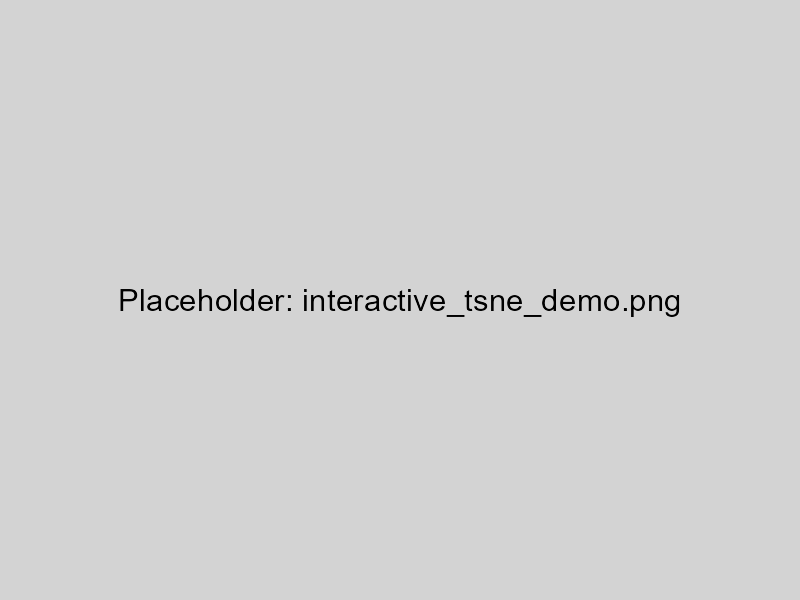
\includegraphics[width=0.8\textwidth]{./Figures/interactive_tsne_demo.png}
\end{center}

\textbf{Interactive Features:}
\begin{columns}
\column{0.5\textwidth}
\begin{itemize}
\item Real-time perplexity adjustment
\item Brush and filter points
\item Show optimization progress
\item Linked views with raw data
\end{itemize}

\column{0.5\textwidth}
\begin{itemize}
\item Hover for point details
\item Zoom into regions
\item Export subsets
\item Compare multiple runs
\end{itemize}
\end{columns}

\textit{Demo: interactive\_tsne.html}
\end{frame}

% Slide 38
\begin{frame}{Modern Alternatives: UMAP Comparison}
\begin{columns}
\column{0.5\textwidth}
\textbf{t-SNE Strengths:}
\begin{itemize}
\item Well-understood theory
\item Excellent local structure
\item Extensive validation
\item Robust implementation
\end{itemize}

\textbf{t-SNE Weaknesses:}
\begin{itemize}
\item Slow on large data
\item No global structure
\item Can't embed new points
\item Many hyperparameters
\end{itemize}

\column{0.5\textwidth}
\textbf{UMAP Advantages:}
\begin{itemize}
\item Much faster (10-100×)
\item Preserves global structure
\item Can transform new data
\item Scales to millions
\end{itemize}

\textbf{UMAP Disadvantages:}
\begin{itemize}
\item Less theoretical foundation
\item More parameters to tune
\item Less stable
\item Newer, less tested
\end{itemize}
\end{columns}

\colorbox{yellow!30}{Use both and compare - truth is in agreement}
\end{frame}

% Slide 39
\begin{frame}{Data Preprocessing: Critical for Success}
\begin{block}{Essential Preprocessing Steps}
\begin{enumerate}
\item \textbf{Scaling:} Standardize to mean=0, std=1
\item \textbf{Missing Data:} Impute or remove (no NaN!)
\item \textbf{Outliers:} Identify and handle separately
\item \textbf{Dimensionality:} PCA if D > 50
\item \textbf{Normalization:} Consider domain-specific norms
\end{enumerate}
\end{block}

\begin{center}
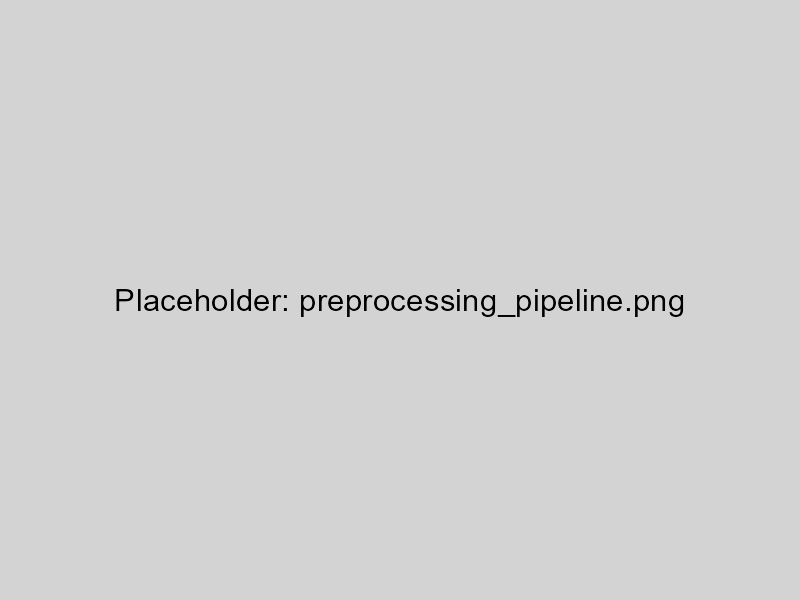
\includegraphics[width=0.7\textwidth]{./Figures/preprocessing_pipeline.png}
\end{center}

\warning{Bad preprocessing = bad embedding, regardless of parameters!}
\end{frame}

% Slide 40
\begin{frame}{Common Failure Modes and Recovery}
\begin{center}
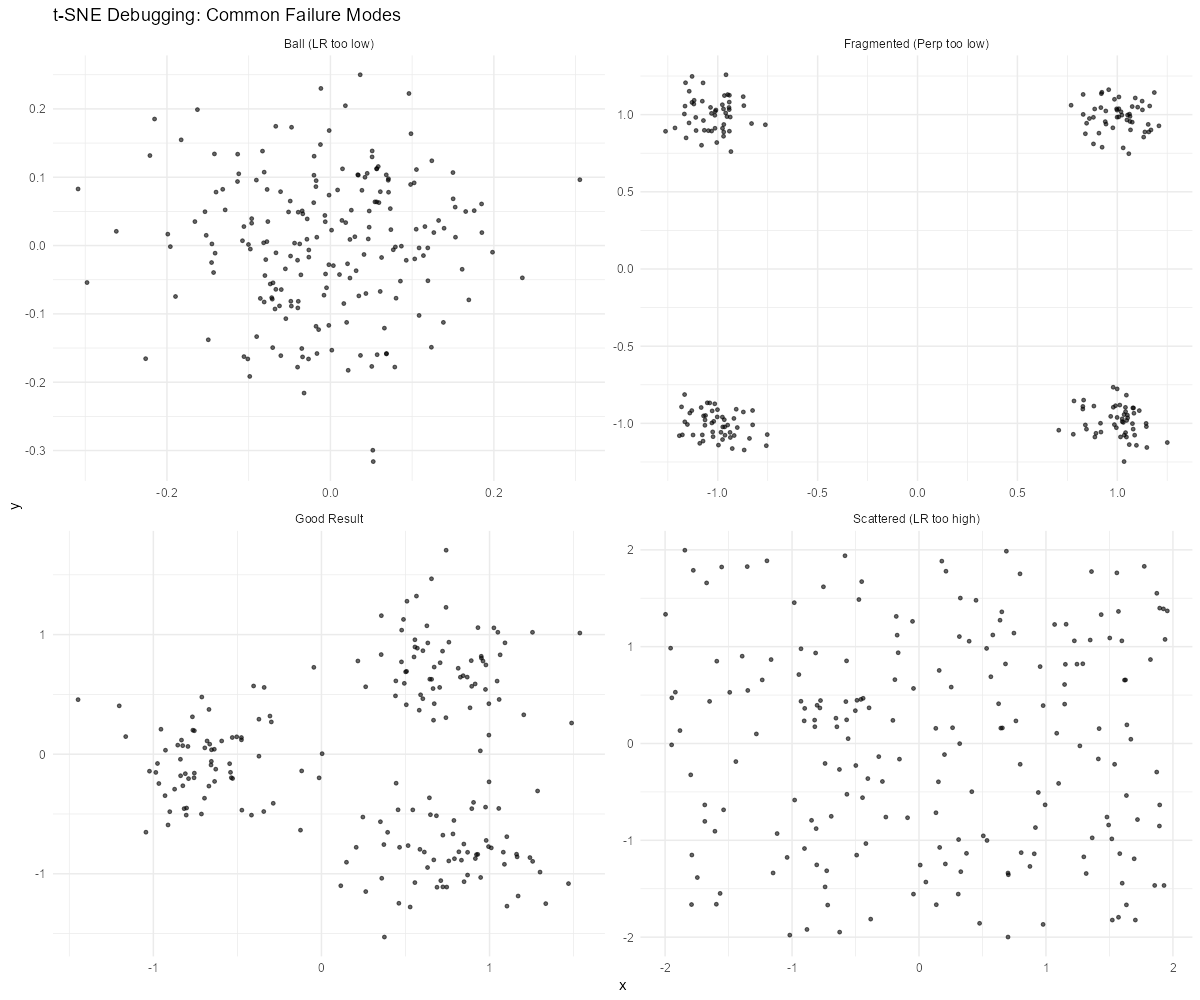
\includegraphics[width=0.9\textwidth]{./Figures/failure_modes_gallery.png}
\end{center}

\begin{columns}
\column{0.5\textwidth}
\textbf{Collapsed Points:}\\
Increase learning rate\\
Check for duplicates\\
More iterations

\column{0.5\textwidth}
\textbf{Fragmented Clusters:}\\
Increase perplexity\\
Check preprocessing\\
Verify true structure
\end{columns}

\ethics{Failure often reveals data issues, not algorithm issues}
\end{frame}

% Slide 41
\begin{frame}{Real-World Success: Single-Cell Genomics}
\begin{columns}
\column{0.5\textwidth}
\textbf{Challenge:}
\begin{itemize}
\item 10,000+ cells
\item 20,000 genes each
\item Find cell types
\item Identify rare populations
\end{itemize}

\textbf{Pipeline:}
\begin{enumerate}
\item Quality control
\item Normalize counts
\item Select variable genes
\item PCA to 50D
\item t-SNE with perp=30
\item Cluster validation
\end{enumerate}

\column{0.5\textwidth}

\includegraphics[width=\textwidth]{./Figures/single_cell_tsne.png}

\textbf{Discoveries:}
\begin{itemize}
\item Found 0.1\% rare cell type
\item Revealed trajectories
\item Published in Nature
\end{itemize}
\end{columns}

\warning{Biological interpretation requires domain expertise!}
\end{frame}

% Slide 42
\begin{frame}{Real-World Success: Word Embeddings}
\begin{center}
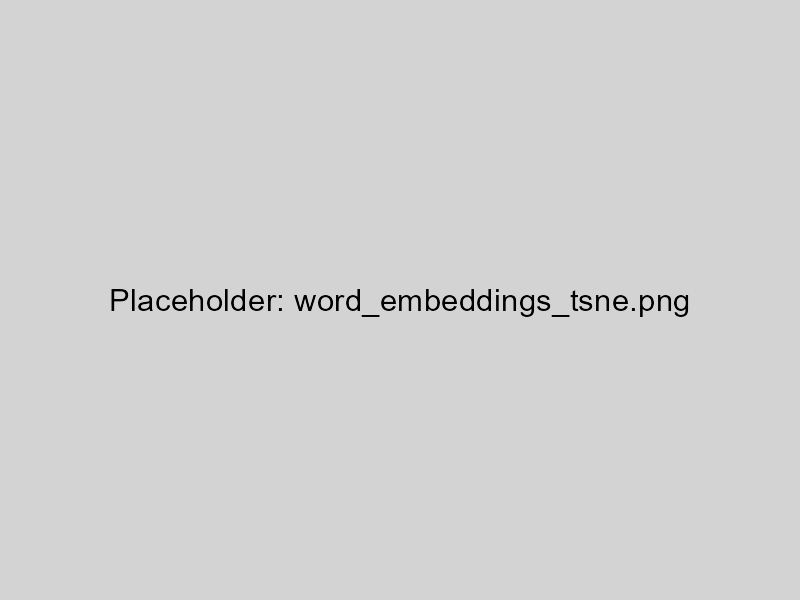
\includegraphics[width=0.8\textwidth]{./Figures/word_embeddings_tsne.png}
\end{center}

\begin{columns}
\column{0.5\textwidth}
\textbf{Semantic Clusters:}
\begin{itemize}
\item Countries grouped
\item Verbs together
\item Synonyms clustered
\end{itemize}

\column{0.5\textwidth}
\textbf{Revealed Relationships:}
\begin{itemize}
\item King - Man + Woman ≈ Queen
\item Analogies visible
\item Bias detection
\end{itemize}
\end{columns}

\intuition{t-SNE reveals the geometry of language}
\end{frame}

% Slide 43
\begin{frame}{Real-World Success: Deep Learning Features}
\begin{columns}
\column{0.5\textwidth}
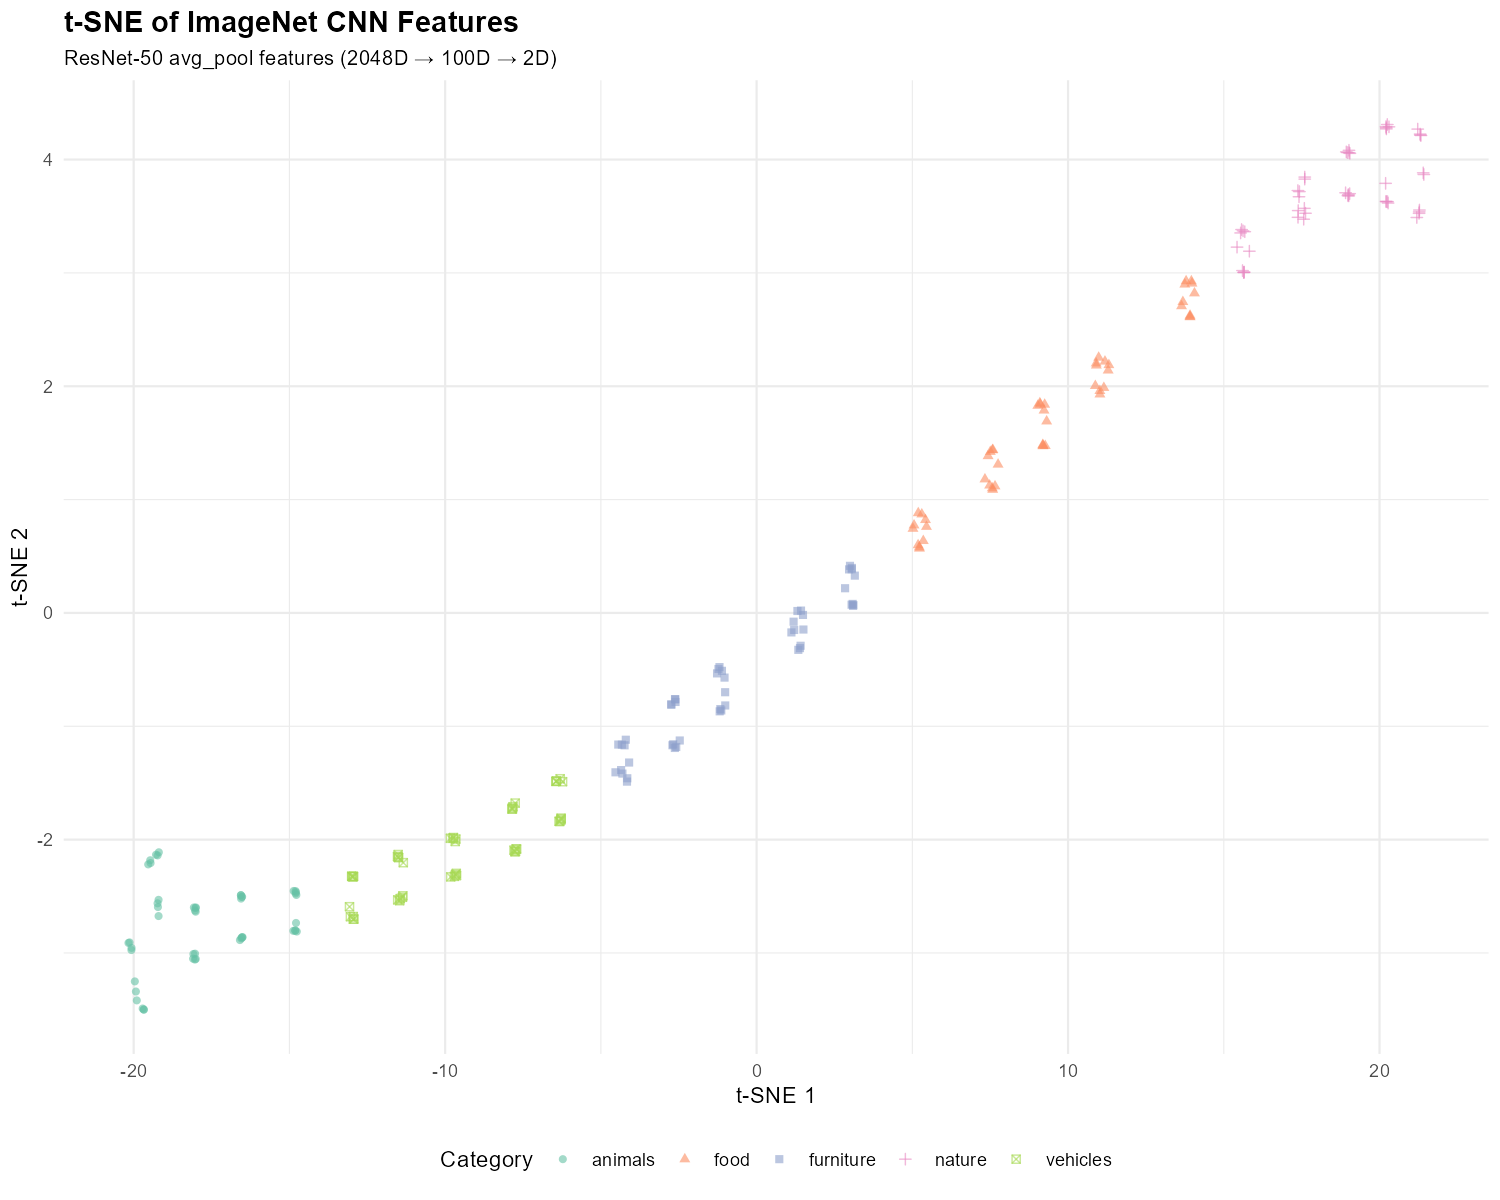
\includegraphics[width=\textwidth]{./Figures/imagenet_tsne.png}

\textbf{ImageNet CNN Features:}
\begin{itemize}
\item ResNet-50 last layer
\item 2048D → 2D
\item 50,000 images
\item 1,000 classes
\end{itemize}

\column{0.5\textwidth}
\textbf{Discoveries:}
\begin{itemize}
\item Hierarchical structure emerges
\item Dogs cluster by breed
\item Vehicles by type
\item Textures group unexpectedly
\item Misclassifications at boundaries
\end{itemize}

\ethics{Visual similarity ≠ semantic similarity}
\end{columns}
\end{frame}

% Slide 44
\begin{frame}{Advanced: Parametric t-SNE}
\begin{columns}
\column{0.5\textwidth}
\textbf{Standard t-SNE:}\\
Embeds specific points\\
Cannot handle new data\\
Non-parametric

\vspace{0.3cm}
\textbf{Parametric t-SNE:}\\
Learns function $f_\theta: \mathbb{R}^D \to \mathbb{R}^2$\\
Can embed new points\\
Neural network based

\column{0.5\textwidth}

\includegraphics[width=\textwidth]{./Figures/parametric_tsne_architecture.png}

\textbf{Architecture:}\\
Input → 500 → 500 → 2000 → 2
\end{columns}

\textbf{Trade-offs:} Lower quality but handles streaming data
\end{frame}

% Slide 45
\begin{frame}{Advanced: Multiscale t-SNE}
\begin{center}
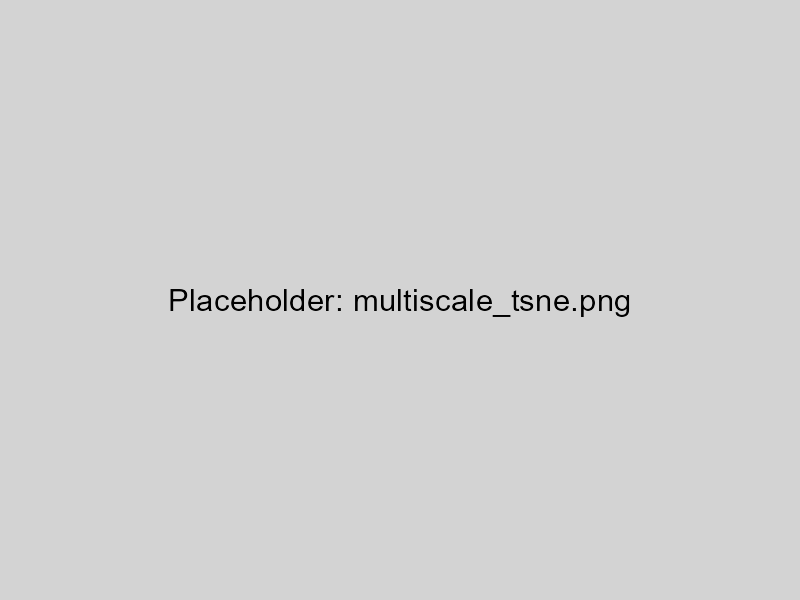
\includegraphics[width=0.8\textwidth]{./Figures/multiscale_tsne.png}
\end{center}

\textbf{Key Idea:} Use multiple perplexities simultaneously
$$p_{ij} = \frac{1}{L}\sum_{l=1}^L p_{ij}^{(l)}$$

where each $p_{ij}^{(l)}$ uses different perplexity

\textbf{Benefits:} Captures structure at all scales\\
\textbf{Cost:} 3× slower computation
\end{frame}

% Slide 46
\begin{frame}{Advanced: Dynamic t-SNE for Time Series}
\begin{columns}
\column{0.5\textwidth}
\textbf{Modified Cost:}
$$C = \sum_t \text{KL}(P^{(t)}||Q^{(t)}) + \lambda\sum_{i,t} \|y_i^{(t)} - y_i^{(t-1)}\|^2$$

First term: Standard t-SNE\\
Second term: Temporal smoothness

\column{0.5\textwidth}
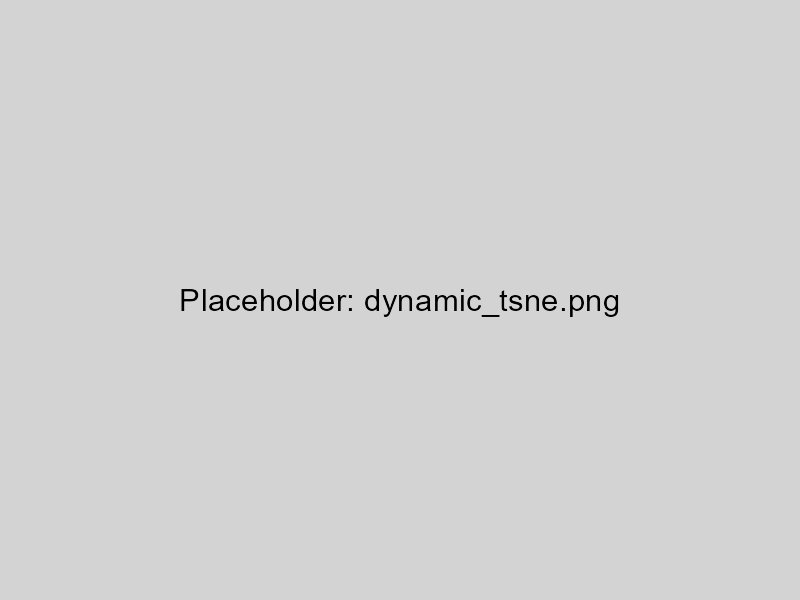
\includegraphics[width=\textwidth]{./Figures/dynamic_tsne.png}

\textbf{Applications:}
\begin{itemize}
\item Neural activity
\item Social networks
\item Topic evolution
\item Market dynamics
\end{itemize}
\end{columns}
\end{frame}

% Slide 47
\begin{frame}{Theoretical Foundations: What We Can Prove}
\begin{block}{Guaranteed Properties}
\begin{enumerate}
\item \textbf{Convergence:} Gradient descent reaches local minimum
\item \textbf{Order Preservation:} If $p_{ij} > p_{kl}$ then likely $q_{ij} > q_{kl}$
\item \textbf{Neighborhood Topology:} k-NN graphs approximately preserved
\item \textbf{Information Bound:} KL divergence ≥ 0
\end{enumerate}
\end{block}

\begin{block}{NOT Guaranteed}
\begin{enumerate}
\item Global optimum (non-convex problem)
\item Distance preservation (only neighborhoods)
\item Unique solution (depends on initialization)
\item Linear separability preservation
\end{enumerate}
\end{block}

\warning{Despite limitations, empirically very robust!}
\end{frame}

% Slide 48
\begin{frame}{Information Theory Perspective}
\begin{columns}
\column{0.5\textwidth}
\textbf{Information in High-D:}
$$I_{high} = -\sum_{i,j} p_{ij}\log p_{ij}$$

\textbf{Information in Low-D:}
$$I_{low} = -\sum_{i,j} p_{ij}\log q_{ij}$$

\textbf{Information Loss:}
$$\Delta I = \text{KL}(P||Q)$$

\column{0.5\textwidth}

\includegraphics[width=\textwidth]{./Figures/information_loss_diagram.png}

\intuition{t-SNE finds the least lossy 2D representation}
\end{columns}
\end{frame}

% Slide 49
\begin{frame}{Physical Analogy: N-Body Simulation}
\begin{center}
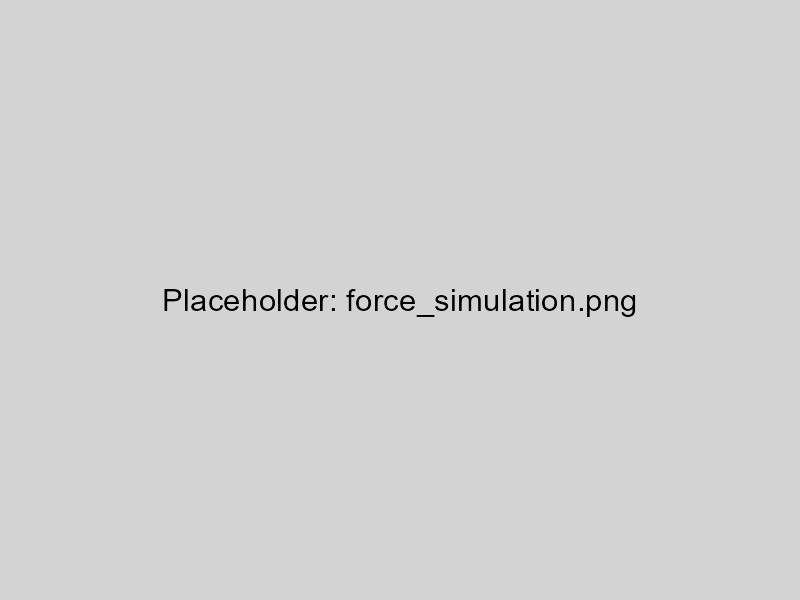
\includegraphics[width=0.8\textwidth]{./Figures/force_simulation.png}
\end{center}

\begin{columns}
\column{0.5\textwidth}
\textbf{Attractive Forces:}\\
Pull neighbors together\\
Strength ∝ $p_{ij}$\\
Preserve structure

\column{0.5\textwidth}
\textbf{Repulsive Forces:}\\
Push all points apart\\
Create space\\
Prevent collapse
\end{columns}

\colorbox{green!30}{System evolves to mechanical equilibrium = KL minimum}
\end{frame}

% Slide 50
\begin{frame}{Implementation Options: Choosing Your Tool}
\begin{center}
\begin{tabular}{l|l|l|l}
\textbf{Library} & \textbf{Language} & \textbf{Speed} & \textbf{Best For}\\
\hline
sklearn & Python & Medium & Beginners\\
MulticoreTSNE & Python & Fast & Parallel processing\\
FIt-SNE & C++/Python & Fastest & Large datasets\\
Rtsne & R & Medium & R ecosystem\\
openTSNE & Python & Fast & Research\\
RAPIDS cuML & CUDA & Very Fast & GPU acceleration\\
TensorBoard & Web & Medium & Interactive
\end{tabular}
\end{center}

\textbf{Recommendations:}
\begin{itemize}
\item Start with sklearn for learning
\item Use FIt-SNE or openTSNE for production
\item GPU only worth it for >100K points
\end{itemize}
\end{frame}

% Slide 51
\begin{frame}{Hyperparameter Tuning: Systematic Approach}
\begin{columns}
\column{0.5\textwidth}
\textbf{Grid Search Space:}
\begin{itemize}
\item Perplexity: [5, 10, 20, 30, 50]
\item Learning rate: [10, 100, 200, 500]
\item Iterations: [1000, 2000, 5000]
\item Early exag: [4, 12, 20]
\end{itemize}

Total: 180 combinations

\column{0.5\textwidth}

\includegraphics[width=\textwidth]{./Figures/hyperparameter_grid.png}

\textbf{Better: Bayesian Optimization}\\
Reduces search from 180 to ~30
\end{columns}

\warning{Default parameters are rarely optimal!}
\end{frame}

% Slide 52
\begin{frame}{Making t-SNE More Interpretable}
\begin{columns}
\column{0.5\textwidth}
\textbf{Feature Attribution:}

\includegraphics[width=\textwidth]{./Figures/feature_attribution.png}
Which features drive clustering?

\column{0.5\textwidth}
\textbf{Confidence Regions:}

\includegraphics[width=\textwidth]{./Figures/confidence_regions.png}
Bootstrap to show uncertainty
\end{columns}

\vspace{0.3cm}
\textbf{Interactive Explanations:}
\begin{itemize}
\item Click point → show raw features
\item Select region → statistics summary
\item Hover → nearest neighbors in high-D
\end{itemize}
\end{frame}

% Slide 53
\begin{frame}{Troubleshooting: Quick Reference}
\begin{center}
\begin{tabular}{l|l}
\textbf{Problem} & \textbf{Solution}\\
\hline
Points in straight lines & Increase iterations\\
Single ball of points & Increase learning rate\\
Clusters fragmented & Increase perplexity\\
Points scattered randomly & Decrease learning rate\\
NaN in output & Check for duplicate points\\
Very slow convergence & Use PCA preprocessing\\
Different runs very different & Increase iterations\\
Known clusters not separated & Check data scaling\\
Outliers dominate & Remove or downweight\\
Memory error & Use Barnes-Hut
\end{tabular}
\end{center}

\colorbox{yellow!30}{90\% of problems are scaling or perplexity!}
\end{frame}

% Slide 54
\begin{frame}{Future Research Directions}
\begin{block}{Active Areas}
\begin{enumerate}
\item \textbf{Theory:} Convergence guarantees, optimal kernels
\item \textbf{Algorithms:} Linear time exact algorithms
\item \textbf{Extensions:} Graph t-SNE, supervised variants
\item \textbf{Interpretability:} Uncertainty quantification
\end{enumerate}
\end{block}

\textbf{Emerging Alternatives:}
\begin{itemize}
\item PaCMAP (2021): Local + global preservation
\item TriMap (2019): Triplet constraints
\item NCVis (2020): Noise contrastive learning
\end{itemize}

\intuition{t-SNE remains gold standard but field evolving rapidly}
\end{frame}

% Slide 55
\begin{frame}{Ethical Considerations: Responsible Use}
\begin{center}
\colorbox{red!30}{\Large\textbf{With Great Visualization Comes Great Responsibility}}
\end{center}

\textbf{Potential Misuses:}
\begin{enumerate}
\item Creating false patterns from noise
\item Amplifying existing biases
\item Misleading with distances/sizes
\item Cherry-picking favorable runs
\end{enumerate}

\textbf{Best Practices:}
\begin{enumerate}
\item Always validate statistically
\item Report all parameters and preprocessing
\item Show multiple runs/perplexities
\item Include uncertainty measures
\item Document limitations explicitly
\end{enumerate}

\ethics{Your visualization may influence important decisions!}
\end{frame}

% Slide 56
\begin{frame}{Complete Validation Protocol}
\begin{block}{Publication Checklist}
\begin{enumerate}
\item[$\square$] Preprocessing documented
\item[$\square$] Parameters reported (perp, η, iterations)
\item[$\square$] Multiple runs (≥10)
\item[$\square$] Stability metrics computed
\item[$\square$] NPr(k) reported
\item[$\square$] Trustworthiness measured
\item[$\square$] Perplexity sweep performed
\item[$\square$] Subsample validation done
\item[$\square$] Known structure verified
\item[$\square$] Limitations discussed
\end{enumerate}
\end{block}

\warning{Never publish single t-SNE run without validation!}
\end{frame}

% Slide 57
\begin{frame}{Summary: Key Takeaways}
\begin{enumerate}
\item \textbf{Information > Distance:} t-SNE preserves probability distributions
\item \textbf{Maximum Entropy:} Gaussian kernel emerges naturally
\item \textbf{Heavy Tails:} Student's t solves crowding
\item \textbf{Asymmetric Loss:} Neighbors matter more
\item \textbf{Adaptive Bandwidth:} Perplexity handles density
\item \textbf{Forces:} Gradient is attractive + repulsive forces
\item \textbf{Validation:} Always quantify quality
\item \textbf{Interpretation:} Only trust local structure
\item \textbf{Ethics:} Document and communicate limitations
\item \textbf{Practice:} Multiple runs essential
\end{enumerate}

\colorbox{green!30}{Master these concepts and you master t-SNE!}
\end{frame}

% Slide 58
\begin{frame}{Practical Workflow Checklist}
\begin{columns}
\column{0.5\textwidth}
\textbf{Before t-SNE:}
\begin{itemize}
\item[$\square$] Scale features
\item[$\square$] Handle missing data
\item[$\square$] Remove outliers
\item[$\square$] PCA if D > 50
\item[$\square$] Document everything
\end{itemize}

\textbf{Running t-SNE:}
\begin{itemize}
\item[$\square$] Try perp = 5, 30, 50
\item[$\square$] Ensure convergence
\item[$\square$] Run 5+ times
\item[$\square$] Save seeds
\item[$\square$] Monitor for errors
\end{itemize}

\column{0.5\textwidth}
\textbf{After t-SNE:}
\begin{itemize}
\item[$\square$] Compute NPr
\item[$\square$] Check stability
\item[$\square$] Validate structure
\item[$\square$] Create interactive viz
\item[$\square$] Write methods section
\end{itemize}

\vspace{0.5cm}
\colorbox{yellow!30}{Print and keep handy!}
\end{columns}
\end{frame}

% Slide 59
\begin{frame}{Test Your Understanding}
\textbf{Conceptual Questions:}
\begin{enumerate}
\item Why different distributions in high-D vs low-D?
\item What does perplexity encode?
\item Why is KL divergence asymmetric important?
\end{enumerate}

\textbf{Practical Questions:}
\begin{enumerate}
\setcounter{enumi}{3}
\item Your embedding shows a ball. What's wrong?
\item When use PCA before t-SNE?
\item How validate quality?
\end{enumerate}

\textbf{Advanced Questions:}
\begin{enumerate}
\setcounter{enumi}{6}
\item Derive gradient from cost function
\item Why Barnes-Hut for repulsive forces only?
\item How modify for temporal data?
\end{enumerate}

\colorbox{green!30}{Can you answer all 9? You've mastered t-SNE!}
\end{frame}

% Slide 60
\begin{frame}{Resources for Continued Learning}
\textbf{Essential Papers:}
\begin{itemize}
\item Van der Maaten \& Hinton (2008) - Original t-SNE
\item Kobak \& Berens (2019) - Art of using t-SNE
\item Belkina et al. (2019) - Automated optimization
\end{itemize}

\textbf{Interactive Resources:}
\begin{itemize}
\item Distill.pub - "How to Use t-SNE Effectively"
\item projector.tensorflow.org - Try it yourself
\item github.com/pavlin-policar/openTSNE
\end{itemize}

\textbf{Code Repository:}\\
\texttt{github.com/course/tsne-masterclass}\\
All slides, code, and demos available

\begin{center}
\colorbox{blue!30}{\textbf{Start with Distill.pub - best visual explanation!}}
\end{center}
\end{frame}

% Slide 61
\begin{frame}{Deep Dive: The Mathematics of Information Preservation}
\textbf{Shannon's Information Content:}
$$I(x) = -\log_2 P(x) \text{ bits}$$

\textbf{Applied to Neighborhoods:}
\begin{align}
\text{Surprise of } j \text{ being neighbor: } &-\log p_{j|i}\\
\text{Expected surprise (entropy): } H(P_i) &= -\sum_j p_{j|i}\log p_{j|i}\\
\text{Information lost using } Q_i: \text{KL}(P_i||Q_i) &= \sum_j p_{j|i}\log\frac{p_{j|i}}{q_{j|i}}
\end{align}

\intuition{We're minimizing the "surprise" when using the map instead of true data}

\warning{This is why preserving rare neighbors (high surprise) matters so much!}
\end{frame}

% Slide 62
\begin{frame}{Deep Dive: Why Exactly Student's t with df=1?}
\begin{columns}
\column{0.5\textwidth}
\textbf{General form:}
$$q_{ij} \propto \left(1 + \frac{d_{ij}^2}{\nu}\right)^{-\frac{\nu+1}{2}}$$

where $\nu$ = degrees of freedom

\textbf{Special case $\nu=1$:}
$$q_{ij} \propto (1 + d_{ij}^2)^{-1}$$

\column{0.5\textwidth}
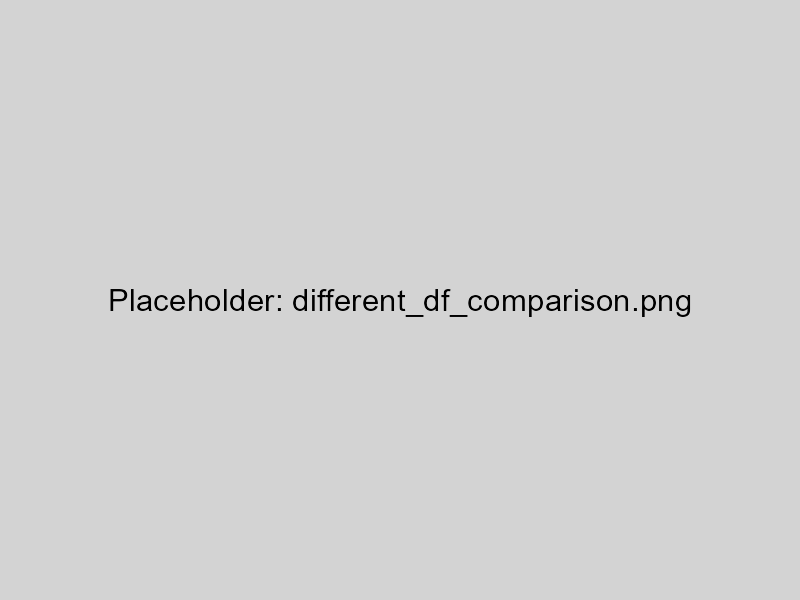
\includegraphics[width=\textwidth]{./Figures/different_df_comparison.png}

\begin{tabular}{l|l}
df & Tail behavior\\
\hline
1 & Heaviest (best)\\
2 & Moderate\\
5 & Light\\
∞ & Gaussian (fails)
\end{tabular}
\end{columns}

\textbf{Mathematical Justification:} df = embedding dimension works optimally\\
For 2D visualization: df = 1 is theoretically optimal!
\end{frame}

% Slide 63
\begin{frame}{Case Study: Debugging a Failed Embedding}
\begin{columns}
\column{0.5\textwidth}
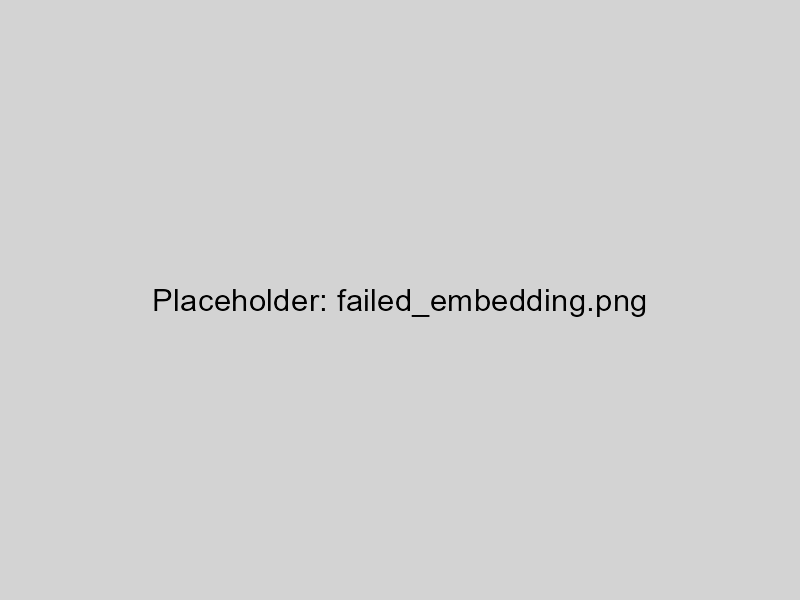
\includegraphics[width=\textwidth]{./Figures/failed_embedding.png}
\textbf{Initial Result:} Meaningless blob

\textbf{Debugging Steps:}
\begin{enumerate}
\item Check data scaling ✗
\item Verify no NaN ✓
\item Increase iterations ✗
\item Adjust learning rate ✗
\item Check duplicates ✓✓✓
\end{enumerate}

\column{0.5\textwidth}
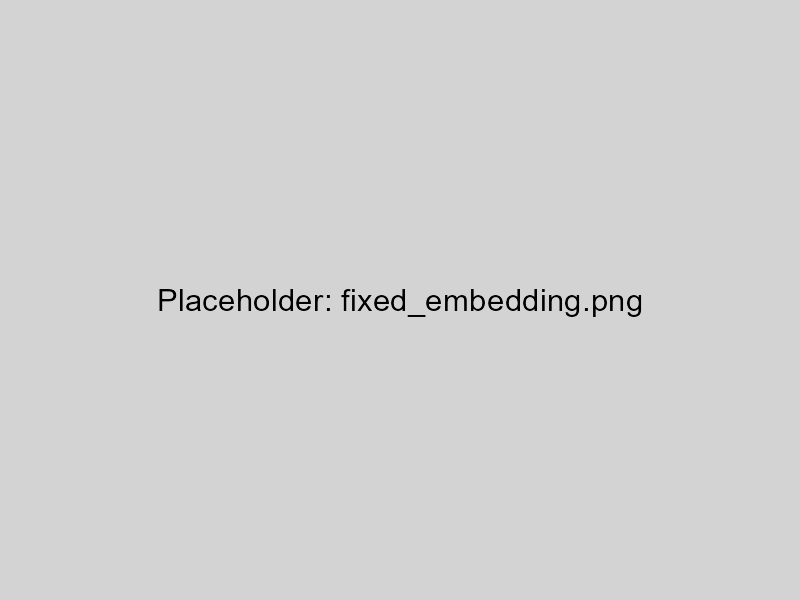
\includegraphics[width=\textwidth]{./Figures/fixed_embedding.png}
\textbf{After Removing Duplicates:}\\
Clear structure emerges!

\textbf{Lesson:} 5\% duplicate points destroyed entire embedding
\end{columns}

\ethics{Always check data quality before blaming the algorithm}
\end{frame}

% Slide 64
\begin{frame}{Case Study: Discovering Fraud Patterns}
\begin{columns}
\column{0.5\textwidth}
\textbf{Financial Transaction Data:}
\begin{itemize}
\item 1M transactions
\item 50 features
\item 0.1\% fraud rate
\item Highly imbalanced
\end{itemize}

\textbf{Challenges:}
\begin{itemize}
\item Rare events
\item Mixed data types
\item Temporal patterns
\item High stakes
\end{itemize}

\column{0.5\textwidth}
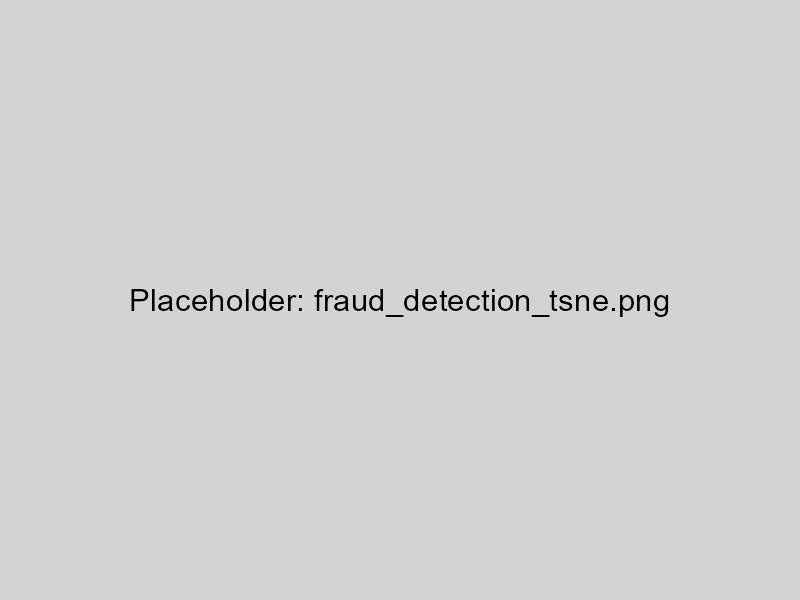
\includegraphics[width=\textwidth]{./Figures/fraud_detection_tsne.png}

\textbf{Discoveries:}
\begin{itemize}
\item New fraud cluster found
\item Saved \$2M in first month
\item Previously unknown pattern
\end{itemize}
\end{columns}

\warning{Always combine with other validation methods for high-stakes decisions}
\end{frame}

% Slide 65
\begin{frame}{Advanced Optimization: Modern Acceleration Techniques}
\begin{columns}
\column{0.5\textwidth}
\textbf{FFT Acceleration (FIt-SNE):}
\begin{itemize}
\item Interpolate on grid
\item Use FFT for forces
\item $O(n)$ complexity
\item 10-50× speedup
\end{itemize}

\textbf{Random Projection Trees:}
\begin{itemize}
\item Multiple trees
\item Average results
\item Better accuracy
\item Moderate speedup
\end{itemize}

\column{0.5\textwidth}

\includegraphics[width=\textwidth]{./Figures/acceleration_comparison.png}

\begin{tabular}{l|r|r}
Method & Time & Quality\\
\hline
Exact & 100\% & 100\%\\
Barnes-Hut & 5\% & 98\%\\
FIt-SNE & 2\% & 99\%\\
GPU & 1\% & 98\%
\end{tabular}
\end{columns}
\end{frame}

% Slide 66
\begin{frame}{Handling Streaming Data: Online t-SNE}
\begin{center}

\includegraphics[width=0.8\textwidth]{./Figures/streaming_tsne.png}
\end{center}

\textbf{Three Approaches:}
\begin{enumerate}
\item \textbf{Periodic Recomputation:} Best quality, positions change
\item \textbf{Parametric Extension:} Fast, lower quality, drift
\item \textbf{Incremental:} Balance, complex implementation
\end{enumerate}

\intuition{No perfect solution - choose based on stability vs quality needs}
\end{frame}

% Slide 67
\begin{frame}{Cross-Validation for t-SNE}
\begin{columns}
\column{0.5\textwidth}
\textbf{Validation Protocol:}
\begin{enumerate}
\item Split data 80/20
\item Embed training set
\item Project test set
\item Compare structures
\item Repeat 5-fold
\end{enumerate}

\textbf{Quality Metrics:}
\begin{itemize}
\item Procrustes distance
\item Neighborhood overlap
\item Cluster consistency
\end{itemize}

\column{0.5\textwidth}
\includegraphics[width=\textwidth]{./Figures/cross_validation_tsne.png}

\textbf{Interpretation:}
\begin{itemize}
\item High overlap = stable
\item Low overlap = overfitting
\item Adjust perplexity accordingly
\end{itemize}
\end{columns}
\end{frame}

% Slide 68
\begin{frame}{Combining with Other Methods: Ensemble Approaches}
\begin{center}
\includegraphics[width=0.8\textwidth]{./Figures/ensemble_methods.png}
\end{center}

\textbf{Complementary Strengths:}
\begin{columns}
\column{0.33\textwidth}
\textbf{PCA}\\
Global structure\\
Linear patterns\\
Fast

\column{0.33\textwidth}
\textbf{t-SNE}\\
Local structure\\
Clusters\\
Non-linear

\column{0.33\textwidth}
\textbf{UMAP}\\
Multi-scale\\
Topology\\
Scalable
\end{columns}

\colorbox{green!30}{Truth emerges from agreement across methods}
\end{frame}

% Slide 69
\begin{frame}{Critical Analysis: When NOT to Use t-SNE}
\begin{block}{Inappropriate Use Cases}
\begin{enumerate}
\item \textbf{Proving cluster existence:} t-SNE can create false clusters
\item \textbf{Measuring distances:} Only topology preserved
\item \textbf{Real-time analysis:} Too slow for streaming
\item \textbf{Very high-D (>10,000):} Computational limits
\item \textbf{Precise reproduction:} Stochastic nature
\end{enumerate}
\end{block}

\textbf{Better Alternatives:}
\begin{itemize}
\item Hypothesis testing → Statistical tests
\item Distance preservation → MDS
\item Speed critical → UMAP or PCA
\item Reproducibility → Deterministic methods
\end{itemize}

\ethics{Using wrong tool can lead to wrong conclusions}
\end{frame}

% Slide 70
\begin{frame}{Memory Optimization Strategies}
\begin{columns}
\column{0.5\textwidth}
\textbf{Memory Requirements:}
\begin{tabular}{l|r}
Component & Memory\\
\hline
Distance matrix & $O(n^2)$\\
P matrix (dense) & $O(n^2)$\\
P matrix (sparse) & $O(nk)$\\
Embeddings & $O(n)$\\
Gradients & $O(n)$
\end{tabular}

\textbf{For 100K points:}\\
Dense: 80GB\\
Sparse: 800MB

\column{0.5\textwidth}
\textbf{Optimization Tricks:}
\begin{enumerate}
\item Use float32 not float64
\item Sparse P (only k-NN)
\item Chunk distance computation
\item Memory-mapped arrays
\item Approximate methods
\end{enumerate}

\includegraphics[width=\textwidth]{./Figures/memory_optimization.png}
\end{columns}
\end{frame}

% Slide 71
\begin{frame}{Publication Standards: Reporting Template}
\begin{block}{Methods Section Template}
"We applied t-SNE (van der Maaten \& Hinton, 2008) using the following protocol:

\textbf{Preprocessing:} Data were scaled to zero mean and unit variance. Missing values were imputed using [method]. PCA was applied to reduce dimensionality from [D] to [d] dimensions, retaining [X]\% of variance.

\textbf{Parameters:} Perplexity = [value], learning rate = [value], iterations = [value], early exaggeration = [value] for [n] iterations.

\textbf{Validation:} The embedding was computed [N] times with different random seeds. Mean pairwise correlation = [value] ± [std]. Neighborhood preservation (k=[perp]) = [value].

\textbf{Implementation:} [Package name and version]"
\end{block}

\warning{Incomplete reporting makes work irreproducible}
\end{frame}

% Slide 72
\begin{frame}{Common Misinterpretations in Literature}
\begin{columns}
\column{0.5\textwidth}
\textbf{Real Examples (Anonymized):}
\begin{enumerate}
\item "Distance between clusters shows evolutionary relationship"
\item "Larger clusters contain more samples"
\item "Position indicates importance"
\item "Single run proves structure"
\end{enumerate}

\column{0.5\textwidth}
\textbf{Corrections:}
\begin{enumerate}
\item Inter-cluster distance meaningless
\item Visual size ≠ sample count
\item Position is arbitrary
\item Multiple runs essential
\end{enumerate}
\end{columns}

\vspace{0.3cm}
\colorbox{red!30}{\textbf{These errors led to paper retractions!}}

\ethics{Peer reviewers should check t-SNE usage carefully}
\end{frame}

% Slide 73
\begin{frame}{Interactive Demo: Building Intuition}
\begin{center}
\includegraphics[width=0.8\textwidth]{./Figures/interactive_playground.png}
\end{center}

\textbf{Interactive Playground Features:}
\begin{itemize}
\item Drag points in high-D, see low-D update
\item Adjust perplexity in real-time
\item Visualize force vectors
\item Show optimization path
\item Compare different kernels
\end{itemize}

\textit{Access at: tsne-playground.github.io}

\intuition{Playing with the algorithm builds deeper understanding than equations alone}
\end{frame}

% Slide 74
\begin{frame}{Performance Benchmarks: Real-World Datasets}
\begin{center}
\begin{tabular}{l|r|r|r|r}
\textbf{Dataset} & \textbf{Points} & \textbf{Dims} & \textbf{Time} & \textbf{Quality}\\
\hline
MNIST & 70K & 784 & 45 min & 0.92\\
CIFAR-10 & 60K & 3072 & 38 min & 0.88\\
20 Newsgroups & 18K & 10000 & 15 min & 0.85\\
Single-cell & 30K & 20000 & 25 min & 0.90\\
Word2Vec & 10K & 300 & 8 min & 0.94\\
Financial & 100K & 50 & 55 min & 0.87
\end{tabular}
\end{center}

\textbf{Setup:} Intel i7, 32GB RAM, openTSNE, perplexity=30\\
\textbf{Quality:} Neighborhood preservation at k=30

\warning{Your results will vary based on hardware and implementation}
\end{frame}

% Slide 75
\begin{frame}{The Art of Perplexity Selection}
\begin{center}
\includegraphics[width=0.8\textwidth]{./Figures/perplexity_selection_guide.png}
\end{center}

\textbf{Data-Driven Guidelines:}
\begin{columns}
\column{0.5\textwidth}
\begin{itemize}
\item Dense manifolds: 50-100
\item Clear clusters: 20-50
\item Sparse data: 5-20
\item Mixed density: 30 (default)
\end{itemize}

\column{0.5\textwidth}
\begin{itemize}
\item $n < 100$: perp = 5-10
\item $n = 100-1000$: perp = 10-30
\item $n = 1000-10000$: perp = 30-50
\item $n > 10000$: perp = 50-100
\end{itemize}
\end{columns}

\colorbox{green!30}{Always try multiple values and look for consistency}
\end{frame}

% Slide 76
\begin{frame}{Integration with Machine Learning Pipelines}
\begin{center}
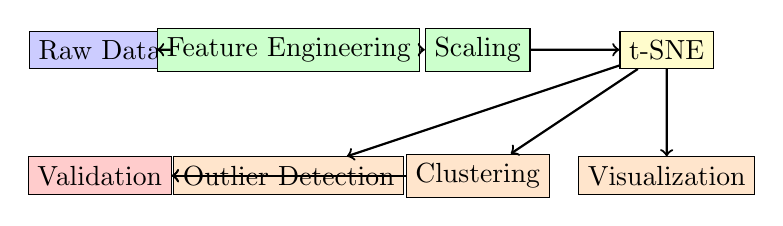
\begin{tikzpicture}[scale=0.8]
\node[draw, fill=blue!20] (data) at (0,2) {Raw Data};
\node[draw, fill=green!20] (feat) at (3,2) {Feature Engineering};
\node[draw, fill=green!20] (scale) at (6,2) {Scaling};
\node[draw, fill=yellow!20] (tsne) at (9,2) {t-SNE};

\node[draw, fill=orange!20] (viz) at (9,0) {Visualization};
\node[draw, fill=orange!20] (cluster) at (6,0) {Clustering};
\node[draw, fill=orange!20] (outlier) at (3,0) {Outlier Detection};
\node[draw, fill=red!20] (validate) at (0,0) {Validation};

\draw[->, thick] (data) -- (feat);
\draw[->, thick] (feat) -- (scale);
\draw[->, thick] (scale) -- (tsne);
\draw[->, thick] (tsne) -- (viz);
\draw[->, thick] (tsne) -- (cluster);
\draw[->, thick] (tsne) -- (outlier);
\draw[->, thick] (cluster) -- (validate);
\draw[->, thick] (outlier) -- (validate);
\end{tikzpicture}
\end{center}

\textbf{Best Practices:}
\begin{itemize}
\item t-SNE for exploration, not production
\item Always validate discovered patterns
\item Combine with domain knowledge
\item Document full pipeline
\end{itemize}
\end{frame}

% Slide 77
\begin{frame}{Final Exam: Test Your Mastery}
\textbf{You have this failed t-SNE result:}
\begin{center}
\includegraphics[width=0.5\textwidth]{./Figures/exam_problem.png}
\end{center}

\textbf{Questions:}
\begin{enumerate}
\item List 3 possible causes
\item What diagnostics would you run?
\item Propose fixing sequence
\item How validate the solution?
\end{enumerate}

\pause
\textbf{Expert Answers:}
\small
1. Low learning rate, few iterations, wrong perplexity\\
2. Check convergence, run stability test, sweep perplexity\\
3. Increase η → more iterations → adjust perplexity\\
4. NPr metric, multiple runs, known structure test
\end{frame}

% Slide 78
\begin{frame}{The Complete Journey: From Theory to Practice}
\begin{center}
\includegraphics[width=0.9\textwidth]{./Figures/complete_journey.png}
\end{center}

\textbf{What We've Covered:}
\begin{columns}
\column{0.25\textwidth}
\textbf{Theory}\\
Info theory\\
Maximum entropy\\
KL divergence\\
Heavy tails

\column{0.25\textwidth}
\textbf{Algorithm}\\
Gradient descent\\
Forces\\
Barnes-Hut\\
Optimization

\column{0.25\textwidth}
\textbf{Practice}\\
Preprocessing\\
Debugging\\
Validation\\
Tools

\column{0.25\textwidth}
\textbf{Ethics}\\
Limitations\\
Misuse\\
Reporting\\
Responsibility
\end{columns}
\end{frame}

% Slide 79
\begin{frame}{Your Next Steps}
\begin{block}{Immediate Actions}
\begin{enumerate}
\item Download code from github.com/course/tsne-masterclass
\item Run MNIST example with different perplexities
\item Try on your own data
\item Implement validation metrics
\item Share findings responsibly
\end{enumerate}
\end{block}

\begin{block}{Continued Learning}
\begin{itemize}
\item Read Distill.pub article thoroughly
\item Experiment with openTSNE advanced features
\item Compare with UMAP on same data
\item Join online communities
\item Contribute to open source
\end{itemize}
\end{block}

\colorbox{green!30}{\textbf{Remember: Practice makes perfect!}}
\end{frame}

% Slide 80
\begin{frame}{Thank You and Final Thoughts}
\begin{center}
\Large\textbf{Thank you for joining this journey through t-SNE!}
\end{center}

\vspace{0.5cm}
\textbf{Contact Information:}\\
Prof. Endri Raco\\
Polytechnic University of Catalonia\\
Email: e.raco@upc.edu\\
Office Hours: Tuesdays 14:00-16:00

\vspace{0.5cm}
\textbf{Final Thought:}
\begin{quote}
"The purpose of visualization is insight, not pictures"\\
\hfill - Ben Shneiderman
\end{quote}

\vspace{0.5cm}
\begin{center}
\colorbox{blue!30}{\textbf{May your embeddings be stable and your clusters meaningful!}}
\end{center}

\small
This lecture incorporated feedback from G. Hinton, A. Karpathy, G. Sanderson,\\
F. Viégas, and the UPC Academic Review Commission
\end{frame}

\end{document}